\appendix
\addcontentsline{toc}{section}{Appendices}

\section*{\LARGE \bfseries Appendix Contents}
\label{sec:appendix_toc}

\par\vspace{0.5em}
\noindent\rule{\textwidth}{0.6pt}
\vspace{0.3em}

\startcontents[appendix]
\printcontents[appendix]{l}{1}{\setcounter{tocdepth}{2}}

\par\vspace{0.3em}
\noindent\rule{\textwidth}{0.6pt}
\vspace{0.5em}

\clearpage


\section{Experiment Details} \label{appx:exp_details}

\begin{table}[htbp]

\caption{Overview of datasets employed in the main body.}
\begin{center}

\scalebox{0.65}{
\begin{tabular}{ccccccc}
\toprule
\textbf{Dataset} & \textbf{Data Size} & \textbf{Input Type} &\textbf{Input Dim ($\mathrm{D}$)} & \textbf{Input ID ($\idx$)} & \textbf{Target Dim} ($n$) & \textbf{Target ID ($\idy$)}\\
\midrule
Swimmer & 20,000 & Raw state & 8 & 3.98 & 2 & 2.00\\

Reacher & 20,000 & Raw state & 11 & 3.65 & 2 & 1.99\\

Hopper & 20,000 & Raw state & 11 & 4.35 & 3  & 2.92\\

Halfcheetah & 20,000 & Raw state & 17 & 6.58 & 6  & 5.27\\

Ant & 20,000 & Raw state & 111 & 7.83 & 8 & 7.43\\

\midrule
MNIST & 50,000 & Grayscale image & 28 $\times$ 28 & 12.76 & 25 & 8.02\\
CIFAR-10 & 50,000 & RGB image & 32$\times$ 32$\times$ 3 & 27.20 & 10 & 9.51\\

\midrule
Cheetah-run & 80,000 & Stacked RGB image & $84\times84\times9$ & 8.96 & 6 & 6.00\\


    
\bottomrule
\end{tabular}
}

\end{center}
\label{table:dataset}
\end{table} 

% \footnotetext{Frame stack is commonly applied for visual control tasks. A single observation is of shape $84\times84\times3$. A frame stack of 3 is used in our experiments, resulting in visual inputs of dimension $84\times84\times9$.}

\subsection{MuJoCo experiments} \label{appx: mujoco}
MuJoCo (Multi-Joint dynamics with Contact) is a physics engine designed for research in robotics, biomechanics, and animation, providing fast and accurate simulations of systems involving complex contact dynamics. It balances physical realism with computational efficiency, enabling reliable modeling of robot–environment interactions \citep{towers2024gymnasium}. Environments involved in this work include:

\begin{itemize}
    \item \textbf{Reacher}: A two-jointed robotic arm tasked with moving its tip to a randomly generated target in a 2D plane. 
    \item \textbf{Swimmer}: A chain-like robot with three body segments connected by two rotors, aiming to propel itself forward in 2D as quickly as possible.
    \item \textbf{Hopper}: A one-legged, four-part robot that seeks to hop forward at maximum speed in 2D.
    \item \textbf{HalfCheetah}: A planar, bipedal robot with a torso and two legs, each consisting of two joints. It aims to run forward as quickly as possible along a 2D track by coordinating its leg movements.
    \item \textbf{Ant}: A quadrupedal robot with four legs and multiple joints, designed to move in a 3D plane. Its goal is to walk or run forward efficiently, despite the challenge of balancing and coordinating many degrees of freedom. Although Ant's state space has 111 dimensions, 84 of the dimensions related to external contact forces are always zeros in the dataset. Thus, the effective input dimension is 27.
\end{itemize}

\begin{figure}[htb]
    \centering
    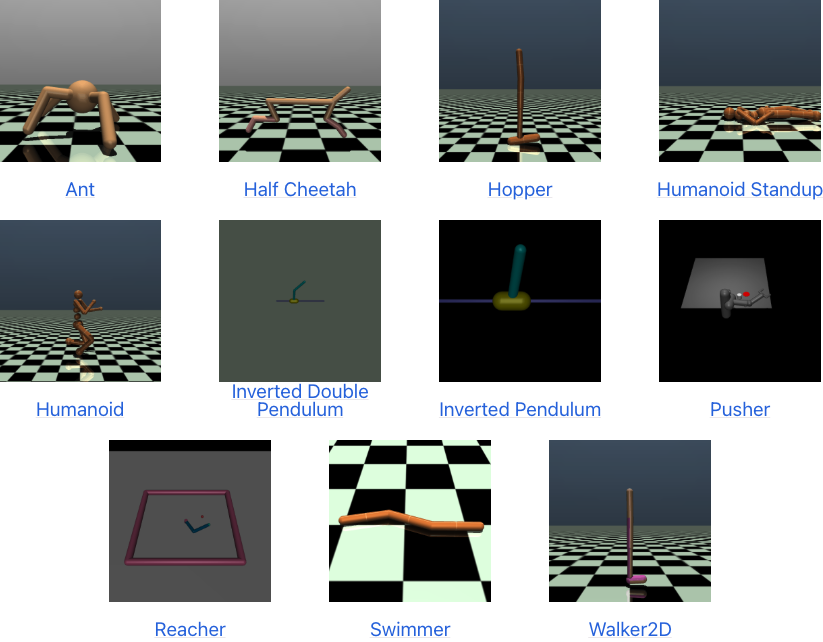
\includegraphics[width=0.6\linewidth]{figures/Appendix/mujoco.png}
    \caption{Screenshot of various MuJoCo environments \citep{towers2024gymnasium}.}
    \label{fig:placeholder}
\end{figure}

All environments introduce stochasticity by perturbing a fixed initial state with Gaussian noise. Their state spaces combine positions of body and joint with corresponding velocities. Control is achieved by applying joint torques, which serve as the actions. Expert datasets are generated by first training policies through online reinforcement learning \citep{fu2020d4rl,gallouedec2024jack} until high performance, then executing these policies to produce trajectories of states $\bx_i$ and actions $\byi$. Here, $\bx_i$ encodes robot positions, joint angles, velocities, and angular velocities, while $\byi$ denotes the applied joint torques.

An episode of expert demonstration has a length of 50 for Reacher, and it has a length of 1,000 for all other environments. Thus, by taking 20,000 data points from each expert dataset, the regression model learns from at least 20 complete trajectories to clone the expert's behavior. For evaluation, we retain a subset of the full validation dataset, keeping the number of data points at 20\% of the training data size. For small datasets (1K) used in Figures~\ref{fig:generalization}, \ref{fig_appx:generalization_appx_1} and \ref{fig_appx:generalization_appx_2}, the test datasets contain 1,000 unseen samples. 

There is no absolute threshold for what constitutes "low-data" versus "high-data," as this depends on problem complexity and data structure. In our experiments, we operationally define this distinction using datasets of 1,000 samples versus 20,000 samples—a 20-fold difference that produces qualitatively different generalization behavior. In the low-data regime, the training set provides sparse coverage of the true data manifold, introducing sampling artifacts such as spurious correlations and outlier effects that do not reflect the true underlying distribution. Models trained on such small datasets, particularly without sufficient regularization, tend to memorize these sample-specific patterns rather than learning generalizable structure. In the high-data regime with 20,000 samples, the training set provides denser coverage, the effect of sampling artifacts diminishes, and the empirical distribution more closely approximates the true underlying distribution.

\begin{table}[h!]
\caption{All hyperparameter settings involved for experiments on MuJoCo datasets. Each figure employs a subset of possible hyperparameter combinations.}
\label{table:mujoco_params}
\vskip 0.15in
\begin{center}
\scalebox{0.7}{
\begin{tabular}{cll}
\toprule
    & \textbf{Hyperparameter} & \textbf{Value}  \\
\midrule
    & Number of hidden layers   & $\{1,2,3,4,5\}$ \\
  Model Architecture  & Hidden layer dimension & $\{64, 128, 256, 512, 1024\}$  \\ 
    & Activation function & ReLU  \\ 
    & Number of linear projection layer ($\bW$) & 1 \\
\midrule
    & Epochs & $3\times10^5$ (20K-datasets) \\
    & & $5\times10^6$ (1K-datasets) \\
    & Batch size & 4096 (20K-datasets) \\
    & & 1000 (1K-datasets) \\
    & Optimizer & SGD \\
    & Learning rate & $1\times10^{-2}$ \\
Training    & Weight decay & $\{0, 10^{-5}, 10^{-4}, 3\times10^{-4}, 5\times10^{-4}, 7\times10^{-4}, 10^{-3}, 3\times10^{-3} \}$, Reacher \\
    &   & $\{0, 10^{-5}, 1/3/5/7\times10^{-4}, 1/3/5/7\times10^{-3}, 10^{-2}, 3\times10^{-2} \}$, Otherwise \\
    & Seed & 0 \\
    & Compute resources & NVIDIA A100 40GB \\
    & Number of CPU compute workers & 4 \\
    & Requested compute memory & 16 GB \\
    & Average training time per model & 20 hours\\
    
\bottomrule
\end{tabular}
}
\end{center}
\end{table} 

Table~\ref{table:mujoco_params} summarizes all model hyperparameters and experimental settings for MuJoCo datasets. A subset of possible hyperparameter combinations is used for each figure:
\begin{itemize}
    \item Figure~\ref{fig:collapse} plots the min-max normalized Test MSE as a function of the min-max normalized NRC1 values for the model architecture 3-256 (3 hidden layers and 256 hidden units) and all possible weight decay values. 
    
      \item Figure~\ref{fig:nrc1_id} establishes the relationship between NRC1 and $\idh$. Each subplot includes all weight decays listed in Table~\ref{table:mujoco_params}. And each weight decay is combined with 9 model architectures in \{3-64, 3-128, 3-256, 3-512, 3-1024, 1-256, 2-256, 4-256, 5-256\}.

      \item Figs.~\ref{fig:generalization}, \ref{fig_appx:generalization_appx_1} and \ref{fig_appx:generalization_appx_2} empirically reveal how generalization ability is affected by $\idh$. We focus on a single model depth of 3, and vary the model width among $\{64, 128, 256, 512\}$. For each model architecture, we evaluate all possible weight decay values listed in Table~\ref{table:mujoco_params}.


    \item Figure~\ref{fig_appx:id_evolution} depict how intrinsic dimension evolves for each network layer. The model architecture is fixed at 3-256 and the title of each subplot annotates the weight decay value.
    
    \item Figure~\ref{fig:6x3_idp1} and \ref{fig:6x3_idp2} follow the same experimental setup as Figs.~\ref{fig:generalization}, \ref{fig_appx:generalization_appx_1} and \ref{fig_appx:generalization_appx_2}, but emphasize on the comparison between $\idh$ and $\idp$.

      \item Figure~\ref{fig_appx:nrc1_wd} record NRC1 values along the training process. The model architecture is fixed to 3-256 for all datasets. And we show 10 weight decay values in $\{0, 0.0001, 0.0003, 0.0005, 0.0007, 0.001, 0.003, 0.005, 0.007, 0.01\}$.
\end{itemize}


\subsection{MNIST/CIFAR10 experiments} \label{appx: vision}
The regression models for both the MNIST and CIFAR-10 tasks were trained across a spectrum of hyperparameters to thoroughly investigate the effects of architecture and regularization on the learned representations. The specific settings for model architecture, optimizer, and other training parameters are detailed in Table 4.


\begin{table}[h!]
  \caption{All hyperparameter settings involved for experiments on MNIST and CIFAR-10 datasets.}
  \label{table:mnist_cifar_params}
  \vskip 0.15in
  \begin{center}
  \scalebox{0.7}{
  \begin{tabular}{cll}
  \toprule
      & \textbf{Hyperparameter} & \textbf{Value}  \\
  \midrule
      & Number of hidden layers  & 3 \\
    Model Architecture  & Hidden layer dimension & $\{32, 64, 128, 256, 512\}$  \\
      & Activation function & ReLU  \\
  \midrule
      & Epochs & 200 \\
      & Batch size & 64 \\
      & Optimizer & Adam \\
      & Learning rate & $\{1 \times 10^{-3}, 5 \times 10^{-3}\}$ \\
  Training    & Weight decay (MNIST) & $\{0, 10^{-5}, 10^{-4}, 3 \times 10^{-4}, 5 \times 10^{-4}, 7 \times 10^{-4}, 10^{-3}, 3 \times
  10^{-3}, 7 \times 10^{-3}\}$ \\
      & Weight decay (CIFAR-10) & $\{0, 10^{-5}, 10^{-4}, 3 \times 10^{-4}, 5 \times 10^{-4}, 7 \times 10^{-4}, 10^{-3}\}$ \\
      & Seed & 0 \\
      & Compute resources & NVIDIA A100 80GB \\
      & Average training time per model & 2 hours\\

  \bottomrule
  \end{tabular}
  }
  \end{center}
  \end{table}

We define noisy-target tasks as tasks where the regression targets contain information that causes models to learn patterns that do not generalize to unseen data. The term "noise" here does not refer to random measurement error or label corruption, but rather to information that varies between semantically similar examples due to instance-specific characteristics rather than reflecting the true underlying function.

The synthetic MNIST regression task represents a low-noise setting. The feature extractor is a CNN trained specifically on MNIST until achieving over 99\% classification accuracy, creating a self-consistent target-generation pipeline. During training, the CNN learns to discard instance-specific variations (such as stroke thickness, slight rotations, or pixel-level noise) that are irrelevant for predicting the target label, retaining only the semantically meaningful information. As a result, the mapping from MNIST images to projected features is smooth and well-aligned with the data domain, enabling models to generalize effectively (Figs.~\ref{fig:generalization} (d),(g)).


In contrast, the synthetic CIFAR-10 regression task is a noisy-target setting due to domain mismatch. CIFAR-10 images are processed through a ResNet-18 pretrained on ImageNet to extract features, which are then projected to 10-dimensional targets. The ImageNet encoder captures fine-grained visual details—texture patterns, color distributions, edge structures—optimized for ImageNet's 1,000 classes. When applied to CIFAR-10's 32×32 images, these features encode not only semantic content but also instance-specific characteristics: two images of cars may differ in color, lighting, rendering artifacts, or background elements, all of which significantly influence the extracted features.
Models can fit these instance-specific components during training, achieving low training error. However, at test time, new images from the same semantic classes exhibit different instance-specific details. The learned mappings for these non-generalizable components do not transfer, resulting in poor generalization. This is evident in Figs.~\ref{fig:generalization} (b),(e), where models achieve low training MSE but high test MSE, characteristic of overfitting to target noise.


\subsection{Visual Control Experiments} \label{appx:vd4rl}
 
Visual D4RL~\citep{lu2023vd4rl} provides offline reinforcement learning benchmarks derived from the DeepMind Control Suite~\citep{tassa2018deepmindcontrolsuite}, where the observations consist of raw RGB pixel inputs rather than proprioceptive states. This introduces additional challenges compared to the state-based MuJoCo tasks described in Appendix~\ref{appx: mujoco}, as the model must extract task-relevant features directly from high-dimensional visual observations while discarding irrelevant visual details.
 
\paragraph{Environment.} We use the Cheetah-run environment, where a planar bipedal robot must run forward as fast as possible. Following standard practice in visual continuous control~\citep{yarats2022drq_v2}, we stack three consecutive $84 \times 84 \times 3$ RGB frames to form $84 \times 84 \times 9$ input tensors, providing temporal context for inferring velocities and dynamics. The target actions are 6-dimensional continuous control commands ($n = 6$). The environment constitutes a Partially Observed Markov Decision Process (POMDP), as individual frames do not fully capture the system state.
 
\paragraph{Datasets.} Expert demonstration datasets are generated by first training policies via online reinforcement learning until high performance, then collecting trajectories of image observations and corresponding actions. We consider two data regimes: 20,000 and 80,000 training samples. Test datasets contain 20,000 samples.
 
\paragraph{Model architecture.} The model consists of two components: a CNN image encoder and an MLP policy network. The encoder contains four convolutional layers, all with 32 output channels and $3 \times 3$ kernels (stride 2 for the first layer, stride 1 for the remaining three), each followed by ReLU activation. Input images are normalized to $[-0.5, 0.5]$, and the encoder outputs a flattened representation of dimension $32 \times 35 \times 35 = 39{,}200$. This representation is passed through a trunk consisting of a linear projection to 50 dimensions, followed by layer normalization and a Tanh activation. The policy head is a 3-hidden-layer MLP with hidden dimension 256 and ReLU activations, followed by a final linear projection layer $\mathbf{W}$ that maps to the 6-dimensional action space. During evaluation, actions are squashed through a $\tanh$ nonlinearity to enforce the $[-1, 1]$ action bounds. The last-layer features $\mathbf{h}$ used for intrinsic dimension and NRC1 analysis correspond to the output of the 3-layer MLP policy head (before the final linear projection $\mathbf{W}$).
 
\paragraph{Training.} Models are trained using the Adam optimizer with a fixed learning rate of $3\times10^{-4}$. The maximum number of training steps is set to $10 \times$ the training data size (e.g., $8 \times 10^5$ steps for the 80K dataset). Weight decay is applied to the network and is varied across a wide range of values:
$
\lambda_{\text{WD}} \in \{0,\; 10^{-5},\; 3 \times 10^{-5},\; 5 \times 10^{-5},\; 7 \times 10^{-5},\; 10^{-4},\; 3 \times 10^{-4},\; 5 \times 10^{-4},\; 7 \times 10^{-4},\; 10^{-3},\; 3 \times 10^{-3},\; 5 \times 10^{-3},\; 7 \times 10^{-3},\; 10^{-2},\; 5 \times 10^{-2},\; 10^{-1}\}
$.
 
\paragraph{Evaluation.} In addition to train and test MSE, we evaluate the learned policies (of 256 hidden dimensions) by executing each of them in the DeepMind Control Suite simulator for $N_{\text{episodes}} = 100$ episodes. Policy performance is reported as a normalized score $\in [0, 100]$ averaged over $N_{\text{episodes}}$ evaluations, obtained by dividing the raw evaluation score by 10 \citep{tarasov2023rebrac}.


\section{Comparison between Regression and Classification} \label{appx:comparison_with_classification}

Previous work on manifold learning for neural classification has demonstrated that the intrinsic dimension of the last hidden layer is negatively correlated with generalization ability. In particular, models achieving lower intrinsic dimension in the penultimate layer were found to exhibit superior test accuracy, with the lowest intrinsic dimension-model attaining the highest top-5 accuracy, see Section 3.2 and Figure 4 in \citet{ansuini2019intrinsic}. 
Additionally, \citet{papyan2020prevalence} connect neural collapse to robust decision boundaries,
\citet{galanti2021role} demonstrate that collapse patterns improve few-shot and transfer learning,
and \citet{li2022understanding} show the degree of collapse in downstream representations strongly predicts transfer accuracy. Complementing these empirical results, there are also theoretical results showing the benefits of neural collapse for classification \citep{gao2023towards,wang2023towards,hui2022limitations}.

In regression, however, our findings indicate a more nuanced picture. We demonstrated the existence of a ``soft" threshold at $\idy$, which delineates distinct generalization regimes. In the under-compressed regime with low-data tasks and high-noise tasks, reducing $\idh$ improves generalization, consistent with the monotonic complexity-performance paradigm observed in classification. However, in the over-compressed regime and in the under-compressed regime with high-data tasks and low-noise tasks, the opposite holds: increasing $\idh$ improves generalization, a phenomenon absent in classification tasks. Thus, in regression, generalization performance depends non-monotonically on the relationship between the learned feature manifold and the intrinsic dimension of the targets.


\section{Intrinsic Dimension and the 2-NN Algorithm} \label{2nnalg}
The intrinsic dimension (ID) of a dataset is the minimum number of coordinates needed to represent the data faithfully. If data points lie on or near a $d$-dimensional manifold $\mathcal{M}$ embedded in $\mathbb{R}^D$ with $d \ll D$, then $d$ is the intrinsic dimension. For example, a circle in 3D space has $d = 1$ and a sphere surface in 10D has $d = 2$.

A critical distinction exists between PCA dimensionality and intrinsic dimension. Consider a 1D spiral embedded in $\mathbb{R}^{10}$ parameterized by $t$. The spiral winds through space with substantial variance across all 10 axes, requiring multiple PCA components to capture the signal. Yet, the intrinsic dimension is exactly $d=1$, because specifying a single scalar value, such as the arc length from the origin, is sufficient to uniquely locate any point on the curve. This illustrates that curved or folded manifolds can require many linear directions to approximate while having low intrinsic dimension. Figure~\ref{fig:nrc_geometry} demonstrates this for neural regression: collapsed features lie near a 2D linear subspace (yellow plane) yet occupy a nonlinear 1D manifold within it.

% Intrinsic dimension has emerged as a powerful tool for quantifying representational capacity in neural networks. \citet{ansuini2019intrinsic} showed that ID evolves systematically across CNN layers, with models achieving lower ID in penultimate layers exhibiting superior generalization. \citet{li2018measuring} used ID to measure the effective dimensionality of parameter spaces, finding that models traversing lower-dimensional solution manifolds generalize better. \citet{pope2021intrinsic} demonstrated that ID of image datasets directly impacts sample complexity, while \citet{yin2024characterizing} recently used per-sample ID to identify untruthful LLM outputs.

We estimate ID using the 2-NN estimator \citep{facco2017estimating}, which exploits a fundamental geometric property: in a $d$-dimensional space, the probability of finding neighbors within a given distance scales with dimension $d$. The key insight is to consider not absolute distances, but the ratio $\mu = r_2/r_1 \geq 1$ of the second to first nearest-neighbor distances. Remarkably, under the assumption of locally uniform density (density approximately constant within the range of the second neighbor), this ratio has a distribution that depends only on the intrinsic dimension $d$, with the local density completely canceling out. Specifically, the cumulative distribution function of $\mu$ is \[F(\mu) = 1 - \mu^{-d}, \quad \mu \geq 1\] 
This property makes the estimator robust to density variations, since we never need to estimate the density itself. Taking logarithms yields the linear relationship \[\log(1 - F(\mu)) = -d \log \mu\]

The 2-NN algorithm estimates $d$ by computing $\mu_i$ for each point, constructing the empirical CDF $F_{\text{emp}}$, and performing linear regression on the transformed coordinates $\{(\log \mu_i, -\log(1 - F_{\text{emp}}(\mu_i)))\}$. The requirement of local uniformity only within the second-neighbor distance is much weaker than global uniformity, making the estimator practical for real datasets with varying density and curvature. 

\begin{algorithm}[H]
\caption{2-NN Intrinsic Dimension Estimation}
\label{alg:2nn}

\KwIn{Dataset $\mathcal{X} = \{\bx_i\}_{i=1}^M$.}
\KwOut{Estimated intrinsic dimension $\hat d$.}

\For{$i \gets 1$ \KwTo $M$}{
  Compute Euclidean distances to the first and second nearest neighbors, $r_1(\bx_i)$ and $r_2(\bx_i)$\;
  
  Compute ratio $\mu_i \gets r_2(\bx_i) / r_1(\bx_i)$\;
}

Sort the ratios such that $\mu_{\sigma(1)} \le \mu_{\sigma(2)} \le \cdots \le \mu_{\sigma(M)}$\;

\For{$i \gets 1$ \KwTo $M$}{
  Assign empirical CDF value $F_{\text{emp}}(\mu_{\sigma(i)}) \gets \frac{i}{M}$\;
}

Construct the coordinate set for regression:
\[
\mathcal{S} \gets \Big\{ \big(\log \mu_{\sigma(i)},\; -\log \!\big(1 - F_{\text{emp}}(\mu_{\sigma(i)})\big)\big) \Big\}_{i=1}^{M-1}
\]

Fit a line through the origin to $\mathcal{S}$ using least squares\;

\Return Slope of the fitted line ($\hat d$)\;

\end{algorithm}


\paragraph{Robustness of the 2-NN estimator.} The robustness of the 2-NN estimator is well justified in the literature and has been widely adopted across various domains~\citep{facco2017estimating, ansuini2019intrinsic, basile2025id_correlation}. It features: (1) the capability to capture intrinsic dimension on nonlinear manifolds; (2) fast computation; and (3) hyperparameter-free estimation. Moreover, as suggested by \citet{facco2017estimating}, we follow the standard block analysis procedure to evaluate the robustness of our ID estimates. The motivation behind block analysis is to distinguish true manifold structure from noise: intrinsic dimensions corresponding to meaningful geometry should remain stable across sample scales, whereas noise-driven dimensions diminish under subsampling. Concretely, we repeatedly estimate ID on progressively smaller random subsets of the data and observe how the estimate changes; a stable plateau indicates genuine intrinsic structure rather than a sampling artifact.

We demonstrate block analyses for two representative cases in Figure~\ref{fig:block_analysis}: (a) non-collapsed Halfcheetah last-layer features and (b) collapsed Ant last-layer features. Block sizes range from 100 to 20{,}000, and for each block size, we subsample 100 times from the training dataset and report the mean and standard deviation of the estimated ID. In both cases, we observe that the ID estimate converges to a stable plateau once the block size exceeds approximately 10{,}000 samples, with diminishing variance as the block size increases. This confirms that the reported ID values reflect true manifold structure rather than finite-sample noise, and that our default subsample size of 18{,}000 lies well within the stable regime.

\begin{figure}[htb]
    \centering
    \subfloat[Non-collapsed Halfcheetah features.]{%
        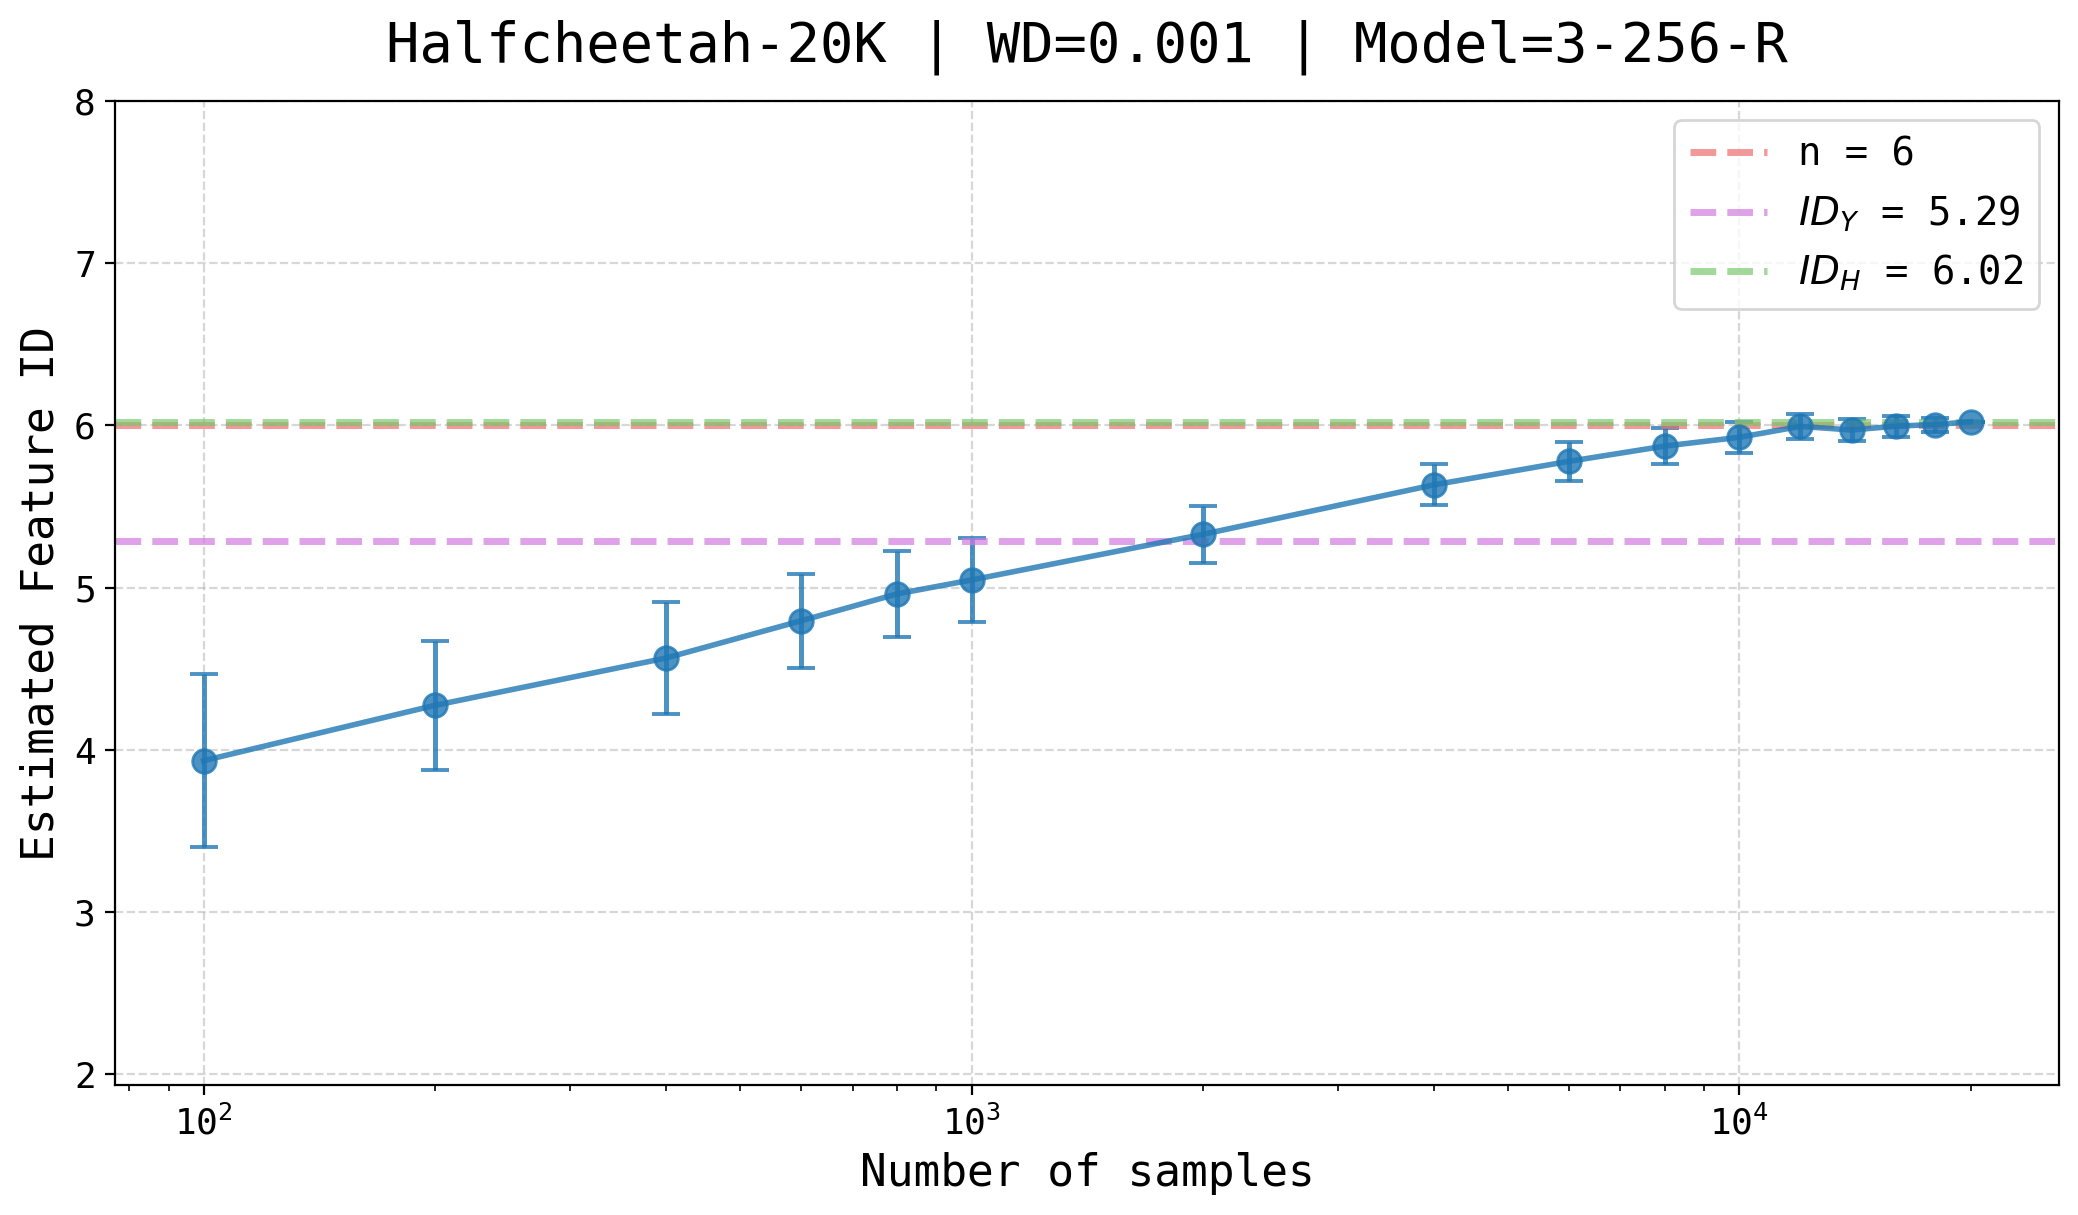
\includegraphics[width=0.48\linewidth]{figures/Appendix/block_analysis_halfcheetah20K.png}%
    }
    \hfill
    \subfloat[Collapsed Ant features.]{%
        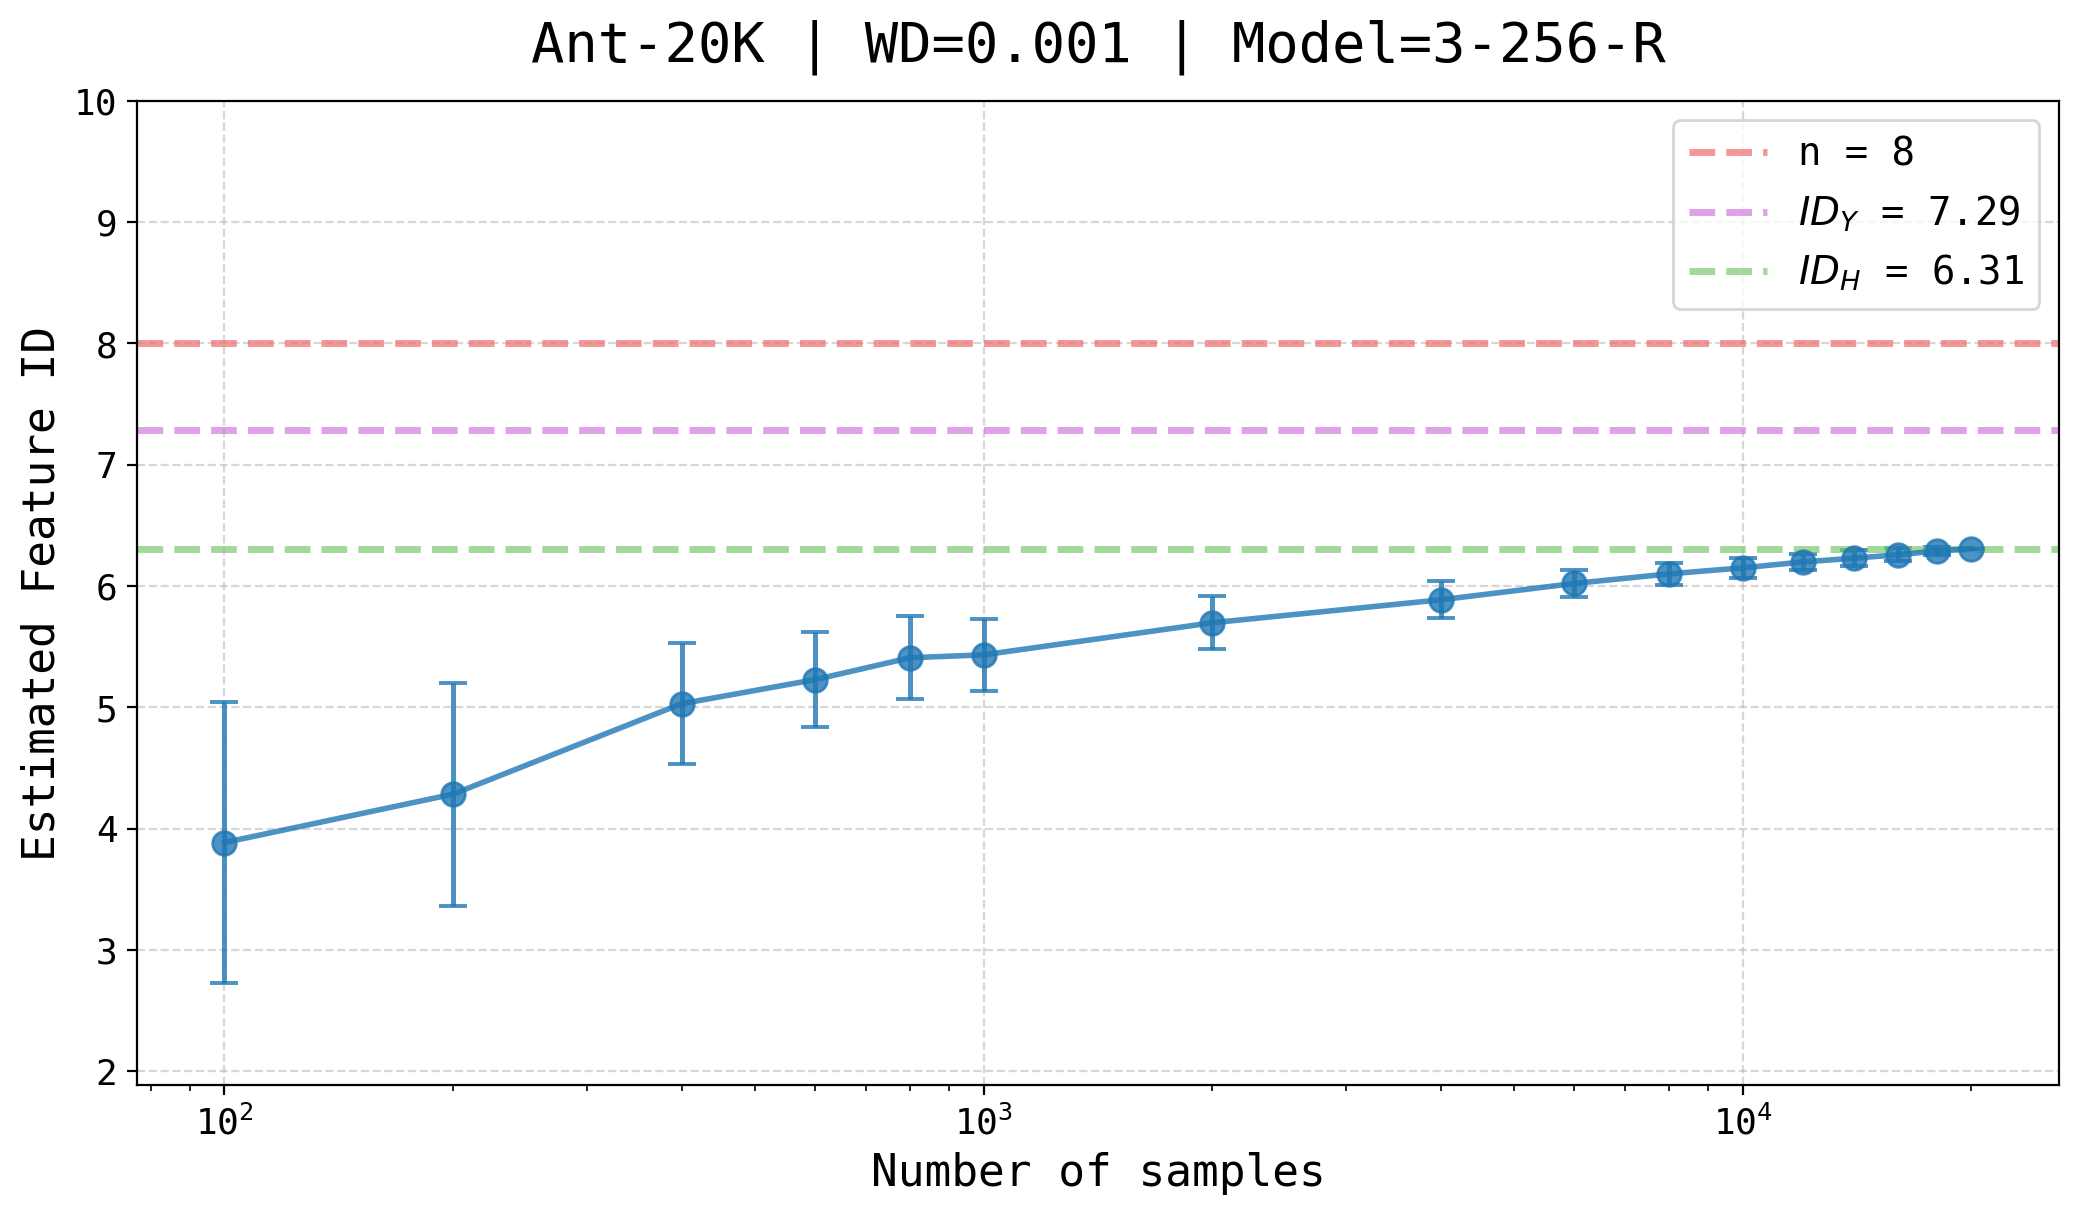
\includegraphics[width=0.48\linewidth]{figures/Appendix/block_analysis_ant20K.png}%
    }
    \caption{Block analysis of the 2-NN intrinsic dimension estimator. Each point shows the mean estimated ID over 100 random subsamples of the given block size. Both cases exhibit a stable plateau for block sizes above approximately 10{,}000, confirming the reliability of the ID estimates at our default subsample size of 18{,}000.}
    \label{fig:block_analysis}
\end{figure}

\section{Evolution of Intrinsic Dimension during Training}
\label{appx: id_evolution}
To further understand the behavior of collapsed models and their counterparts, we track the evolution of the intrinsic dimension throughout training and provide insights. Figure \ref{fig_appx:id_evolution} provides illustrative examples for a collapsed and a non-collapsed model:

\begin{itemize}
    \item For both the collapsed and non-collapsed models, the intrinsic dimension of the last-layer features invariably decreases monotonically until convergence. 
    \item For the collapsed model, the deeper the layer in the network, the lower the intrinsic dimension at the end of training. ReLU activations cause a mild reduction in intrinsic dimension in comparison with the reduction in intrinsic dimension between consecutive layers (ignoring ReLU). Notably, the final intrinsic dimension of the output layer, which gives the actual vector-valued predictions, can be significantly lower than $\idh$.
    \item For non-collapsed models, we usually see --- but not always --- $\idh$ decrease monotonically as we move from shallow to deep layers. Furthermore, we observe that during training, the intrinsic dimension of the output layer hugs the intrinsic dimension of the targets. Thus, tracking the intrinsic dimension of the output layer provides yet another criterion for discriminating between collapsed and non-collapsed models; see Appendix~\ref{appx:output_layer}.  
\end{itemize}

\begin{figure}[htb]
    \centering
    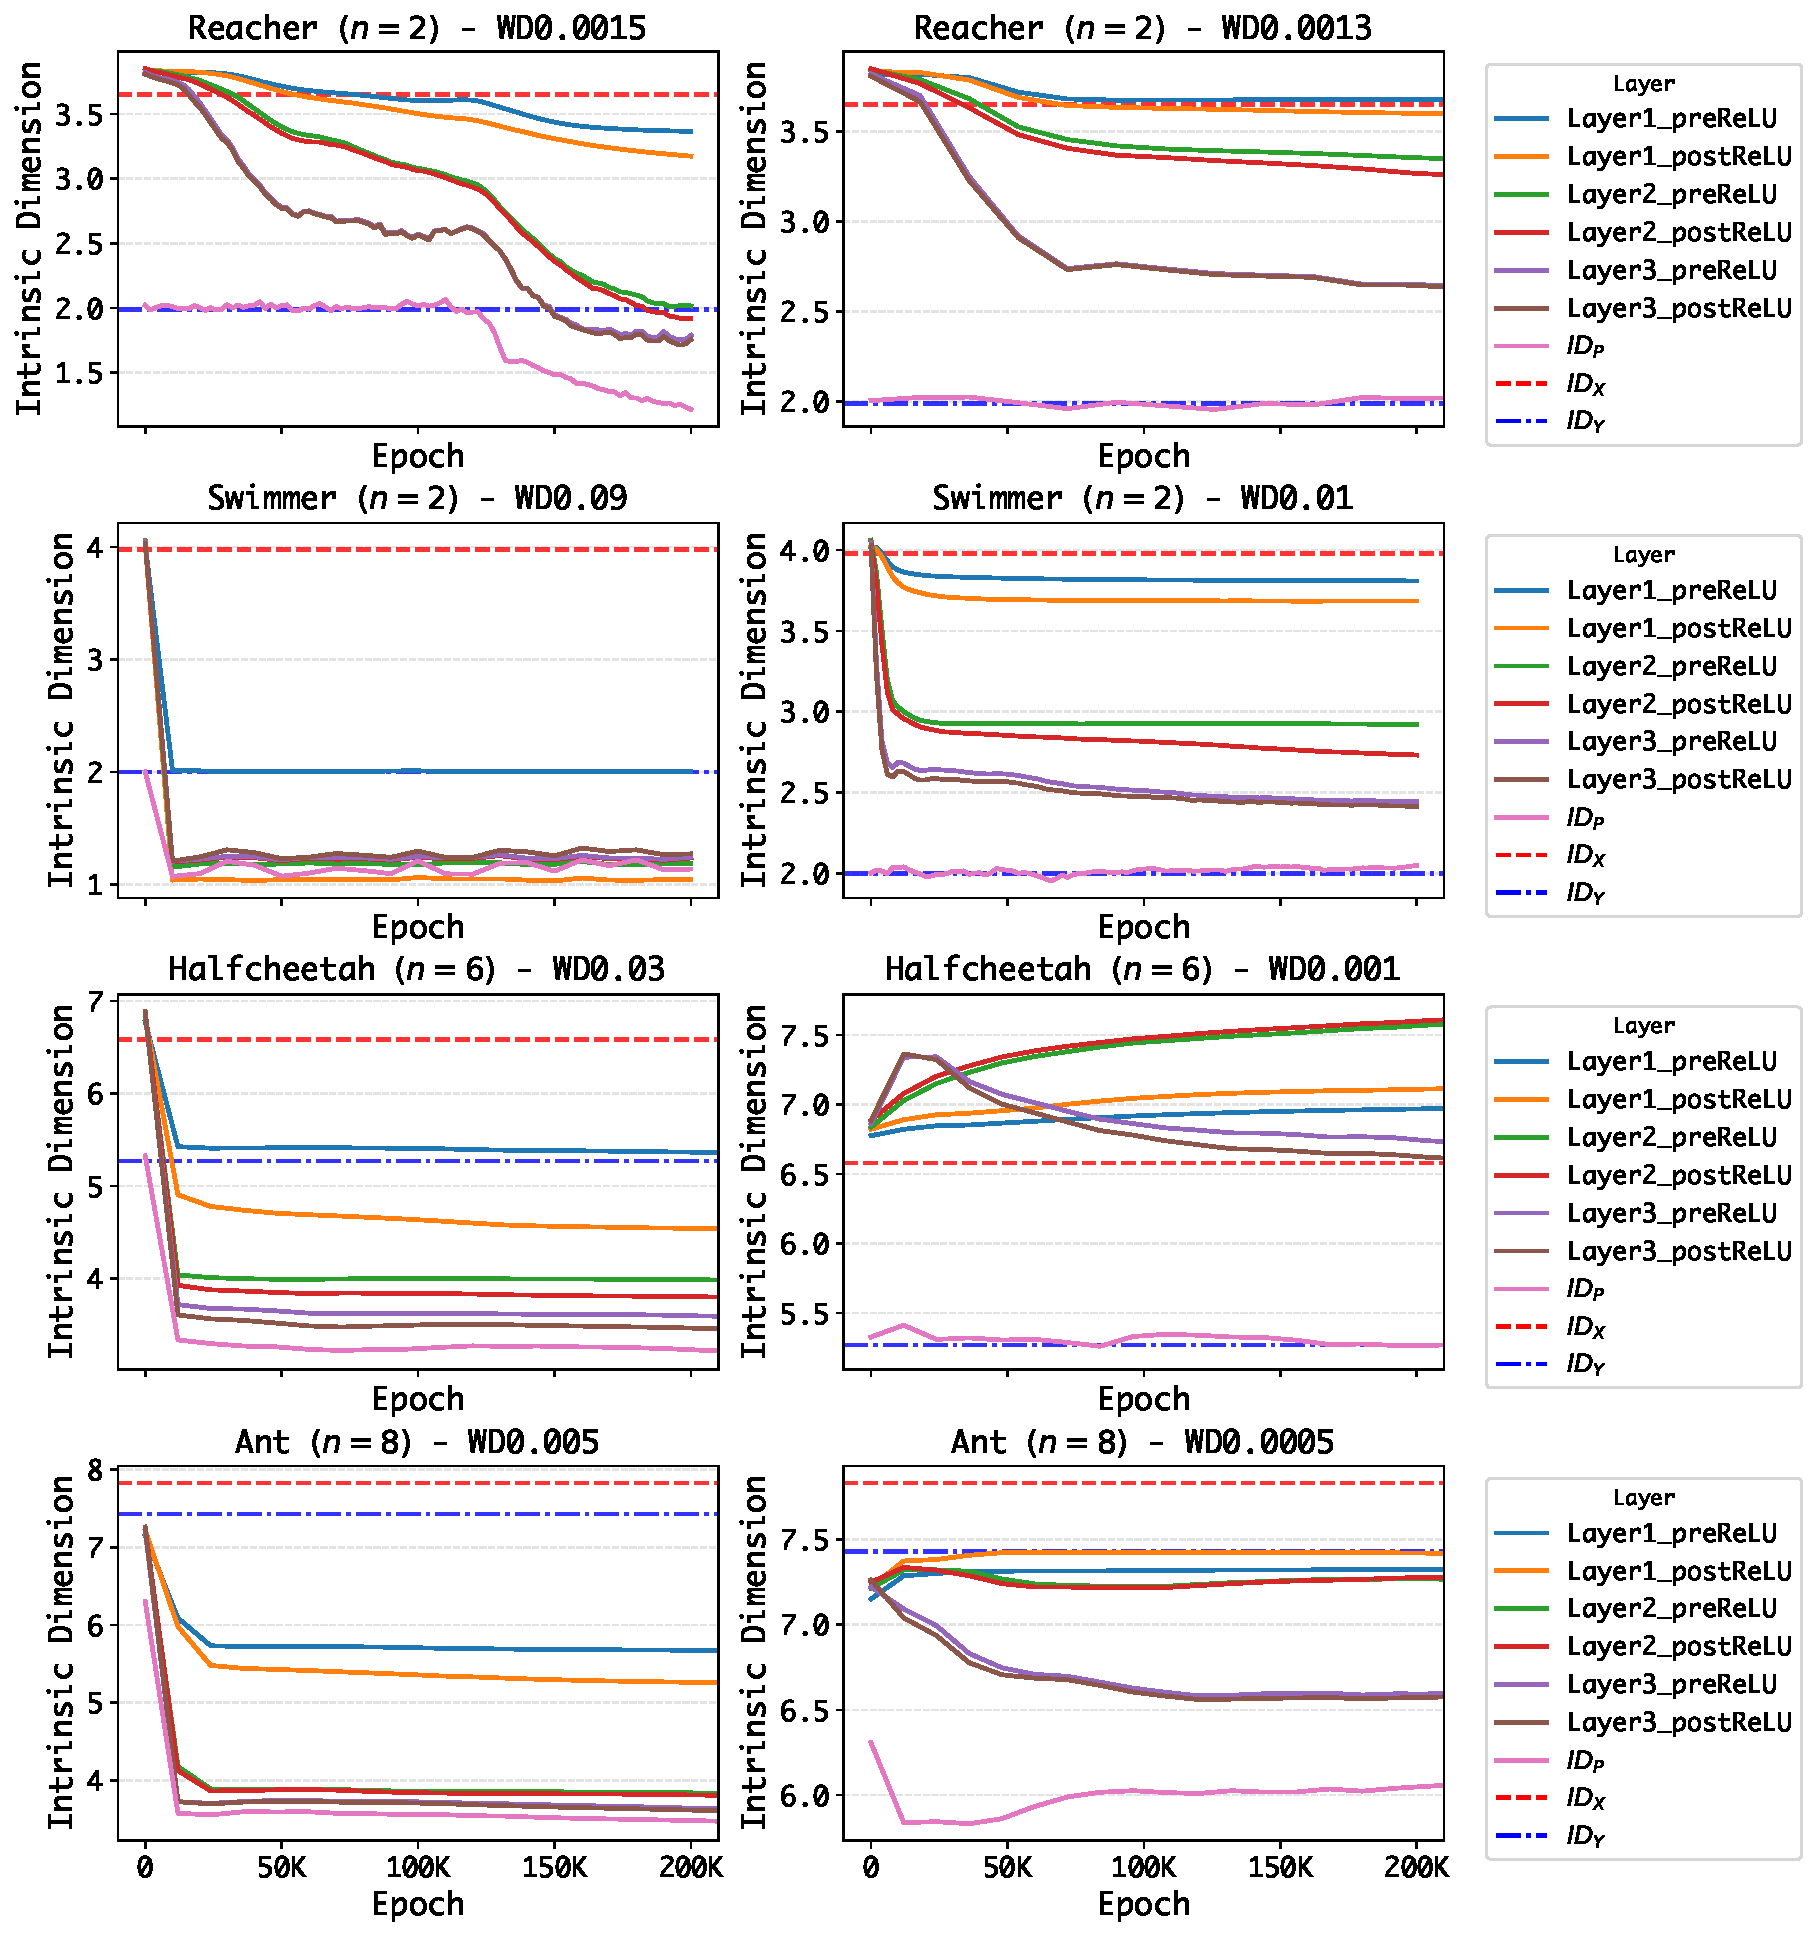
\includegraphics[width=0.8\linewidth]{figures/Appendix/id_evolution.pdf}
    \caption{Intrinsic dimension of input, output, and hidden layers over training epochs for a collapsed (left) and a non-collapsed model (right) for MuJoCo datasets. Each subfigure shows the evolution of intrinsic dimension across layers with blue, red dashed, and pink lines denoting the intrinsic dimension of inputs, targets, and predicted outputs, respectively.}
    \label{fig_appx:id_evolution}
\end{figure}

\newpage
\section{Intrinsic Dimension and Output layer}
\label{appx:output_layer}
We consider here the intrinsic dimension of the outputs (equivalently, the final predictions), $\idp$.
We will see that here too the relationship between intrinsic dimension and generalization exhibits key differences between classification and regression. 

\begin{figure}[htb]
    \centering
    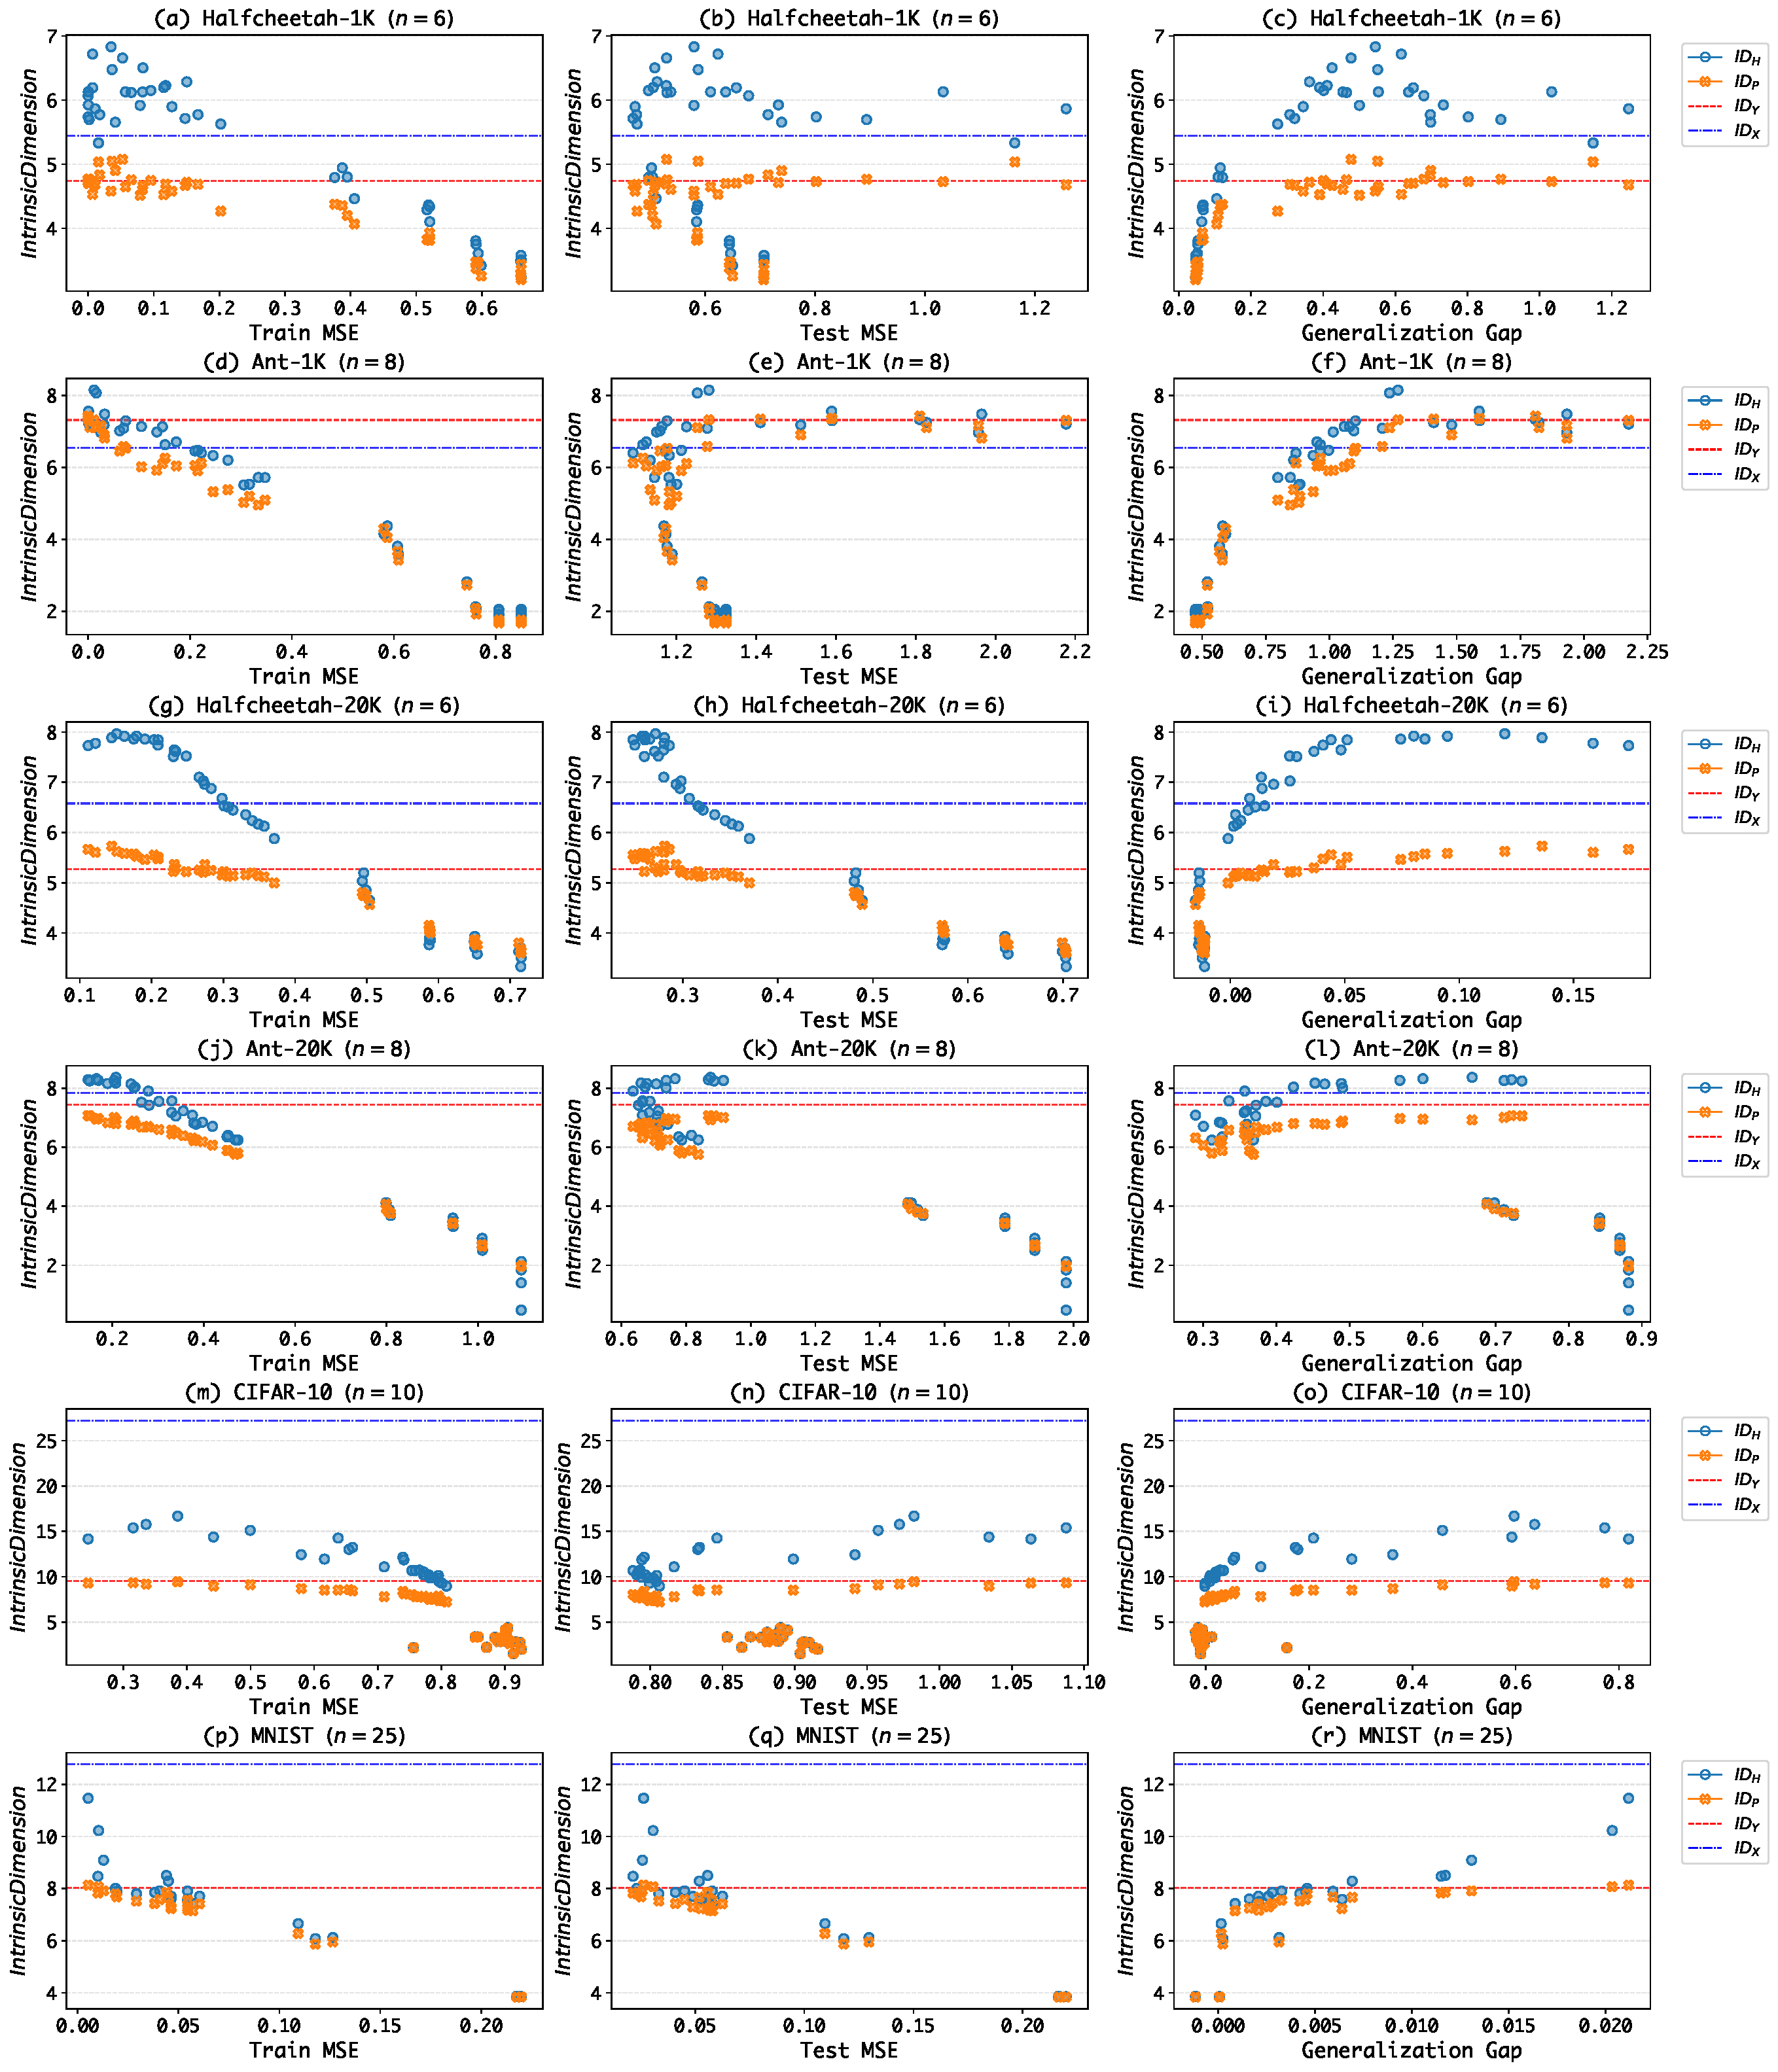
\includegraphics[width=\linewidth]{figures/Appendix/idp1.pdf}
    % \caption{Comparison between $\idh$ and $\idp$.}
    \caption{Comparison between $\idh$ and $\idp$ for Halfcheetah, Ant, CIFAR-10, and MNIST datasets}
    \label{fig:6x3_idp1}
\end{figure}

With respect to the output layer, a structural constraint arises from the classification setting. Specifically, the intrinsic dimension of the output layer necessarily satisfies
\[
\log_2 C\le \idp\le C,
\]
where $C$ is the number of classes. Empirical results consistently show $\idp$ equals the lower bound of this inequality if the model generalizes well. We refer the reader to the discussion in Section 3.1 of \citet{ansuini2019intrinsic}. Conversely, saturation of the upper bound, i.e., $\idp\approx C$, is associated with poor generalization performance, suggesting that maximal output layer dimensionality corresponds to overfitting in classification tasks, see Section 3.5 in \citet{ansuini2019intrinsic}.

In contrast, for neural multivariate regression, the structure of the output leads to the trivial bound
\[
1\le \idp\le n,
\]
where $n$ is the number of output variates. Interestingly, our empirical findings reveal a departure from the classification setting. As shown in the middle column in Figures~\ref{fig:6x3_idp1}-\ref{fig:6x3_idp2}, when the test MSE is low, the intrinsic dimension of the output layer, $\idp$ satisfies $\idp \approx \idy$, which can be close to $n$,  
saturating the upper bound of the inequality above.
Notably, unlike in classification, this saturation is associated with improved test performance. By contrast, when $\idp$ falls below $\idy$, test MSE performance deteriorates, see Figures~\ref{fig:6x3_idp1}-\ref{fig:6x3_idp2}. 


\begin{figure}[htb]
    \centering
    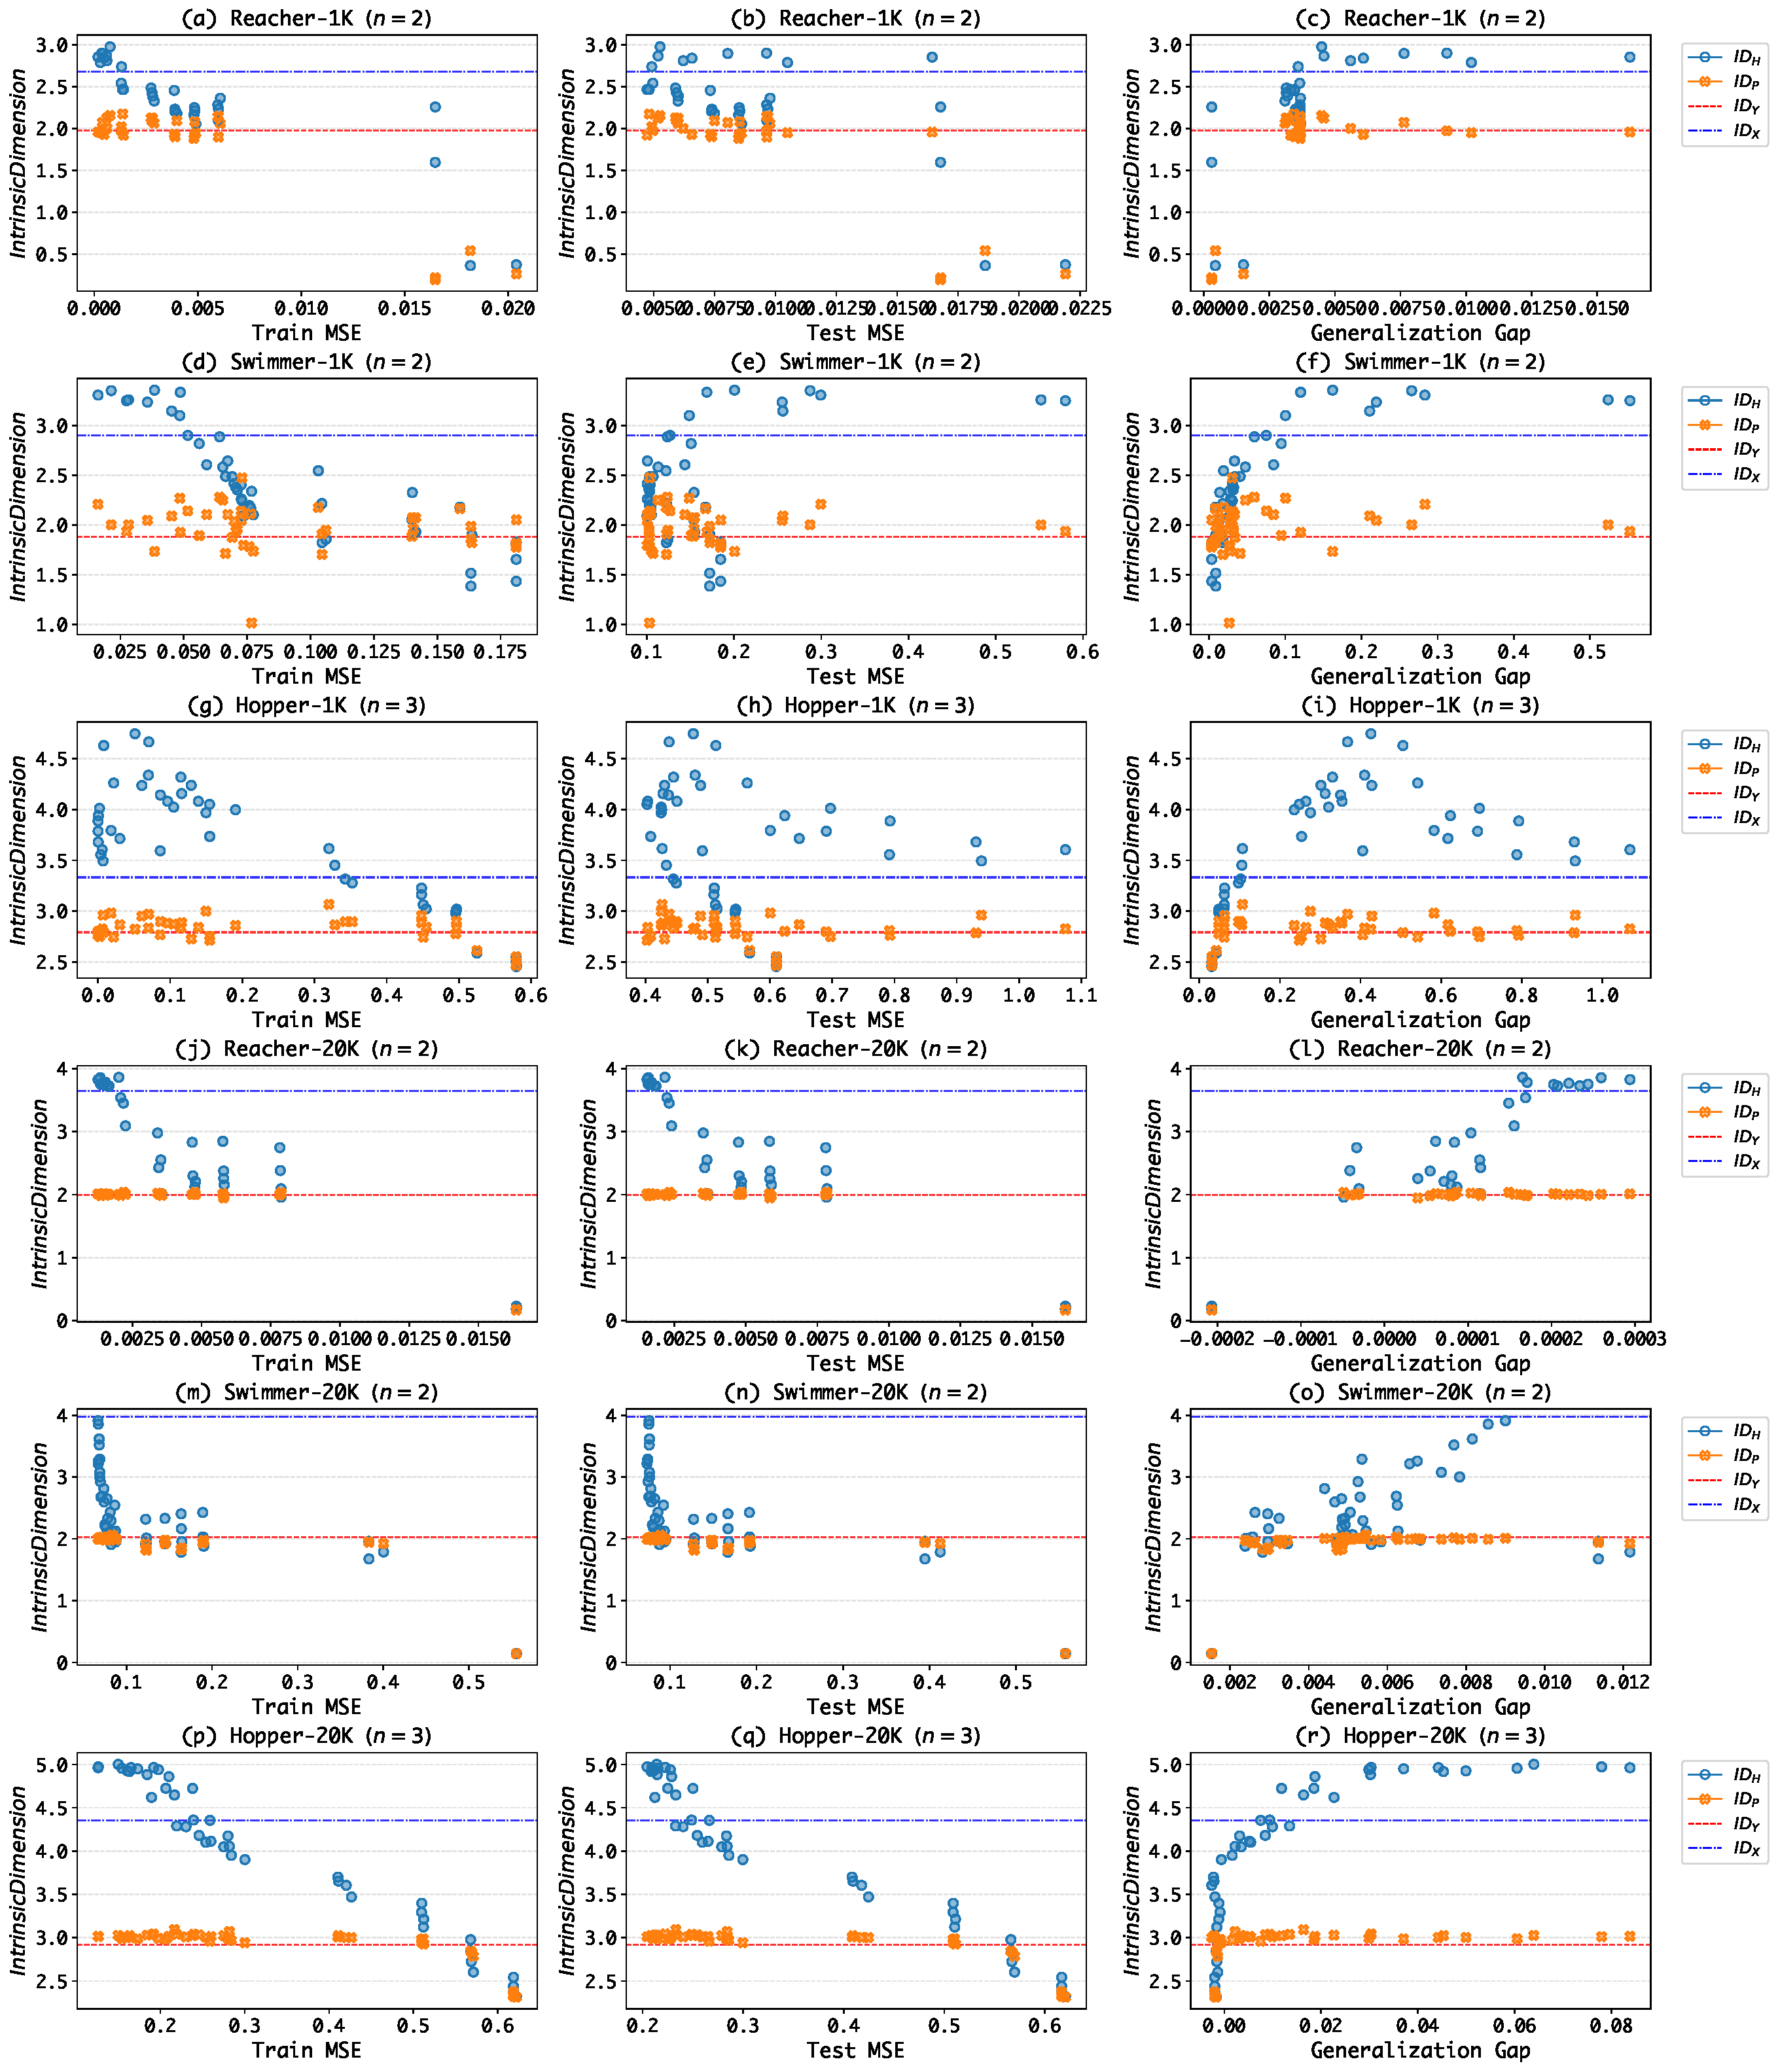
\includegraphics[width=\linewidth]{figures/Appendix/idp2.pdf}
    \caption{Comparison between $\idh$ and $\idp$ for Reacher, Swimmer and Hopper datasets}
    \label{fig:6x3_idp2}
\end{figure}


\clearpage
\section{Additional Experiments on Generalization} 
\label{appx:generalization}

This section lists additional results that complement the experiments in the main body for all considered datasets. Figure~\ref{fig_appx:generalization_appx_1} and ~\ref{fig_appx:generalization_appx_2} shows how generalization power correlates with $\idh$. Our key takeaways are summarized in Table~\ref{table:gen}.


\begin{figure}[htb]
    \centering
    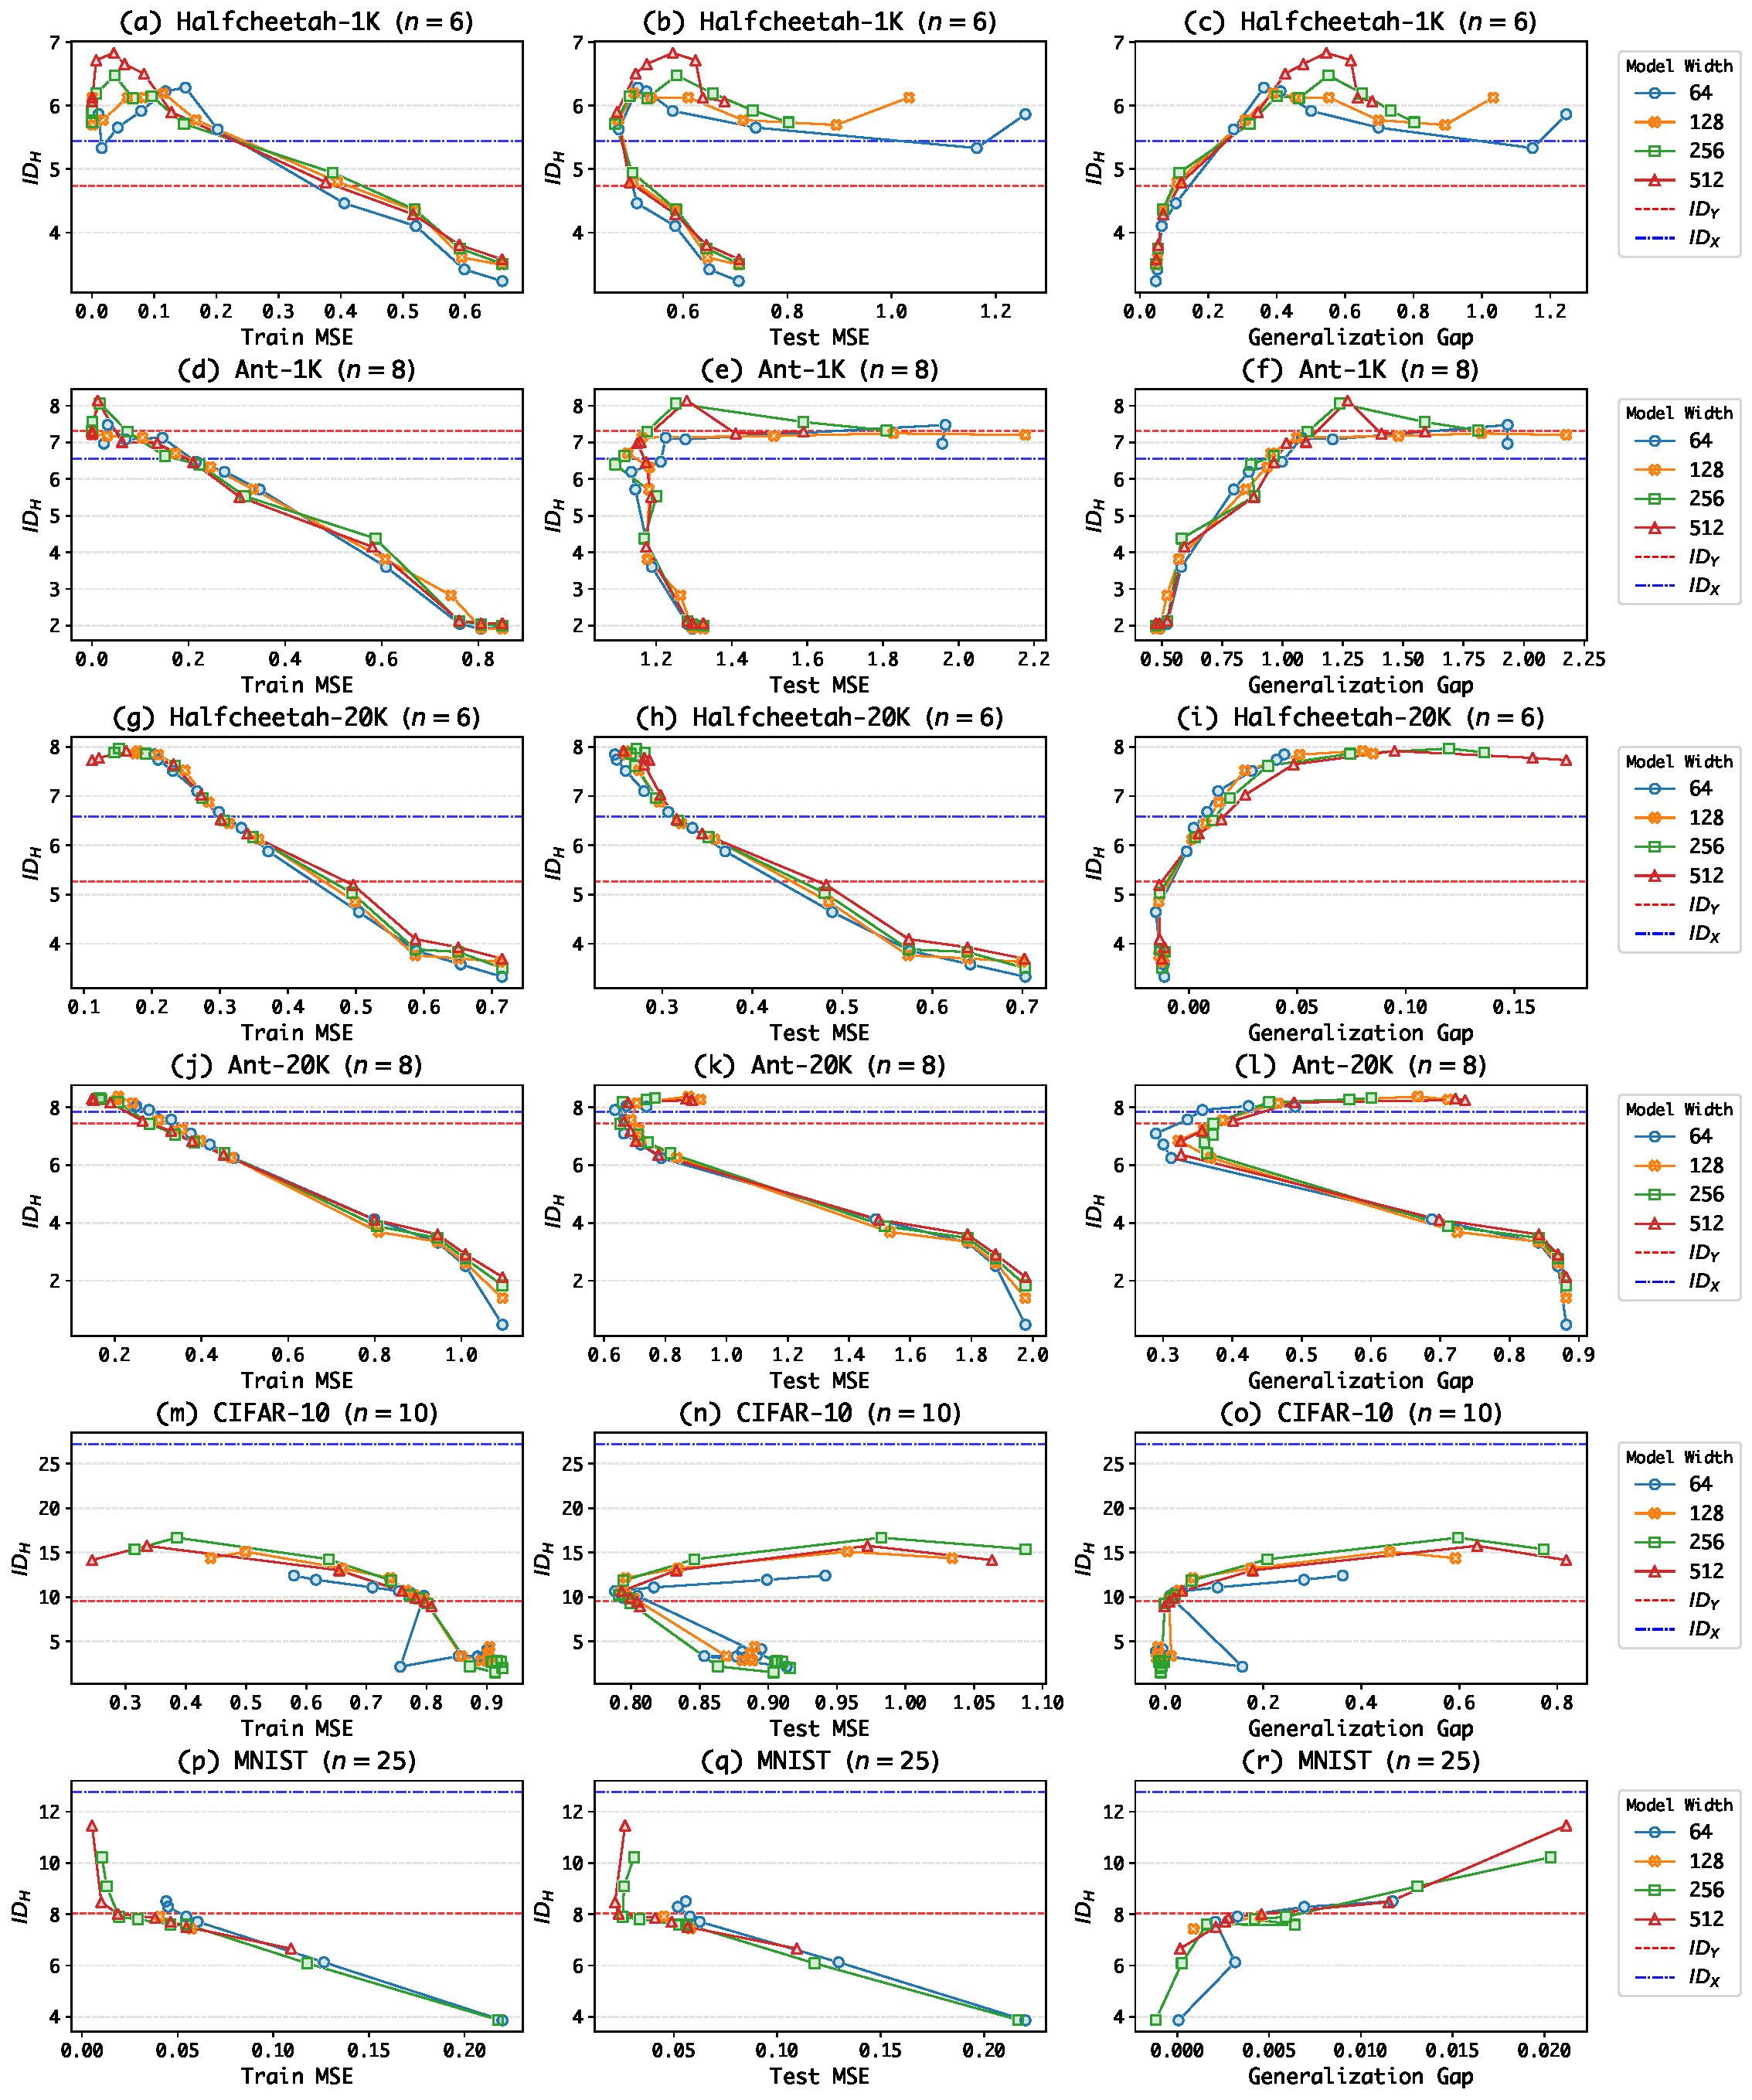
\includegraphics[width=\linewidth]{figures/Appendix/generalization_full_2.pdf}
    \caption{Generalization ability and Intrinsic Dimension for Halfcheetah, Ant, CIFAR-10, and MNIST datasets.}
    \label{fig_appx:generalization_appx_1}
\end{figure}


\begin{figure}[htb]
    \centering
    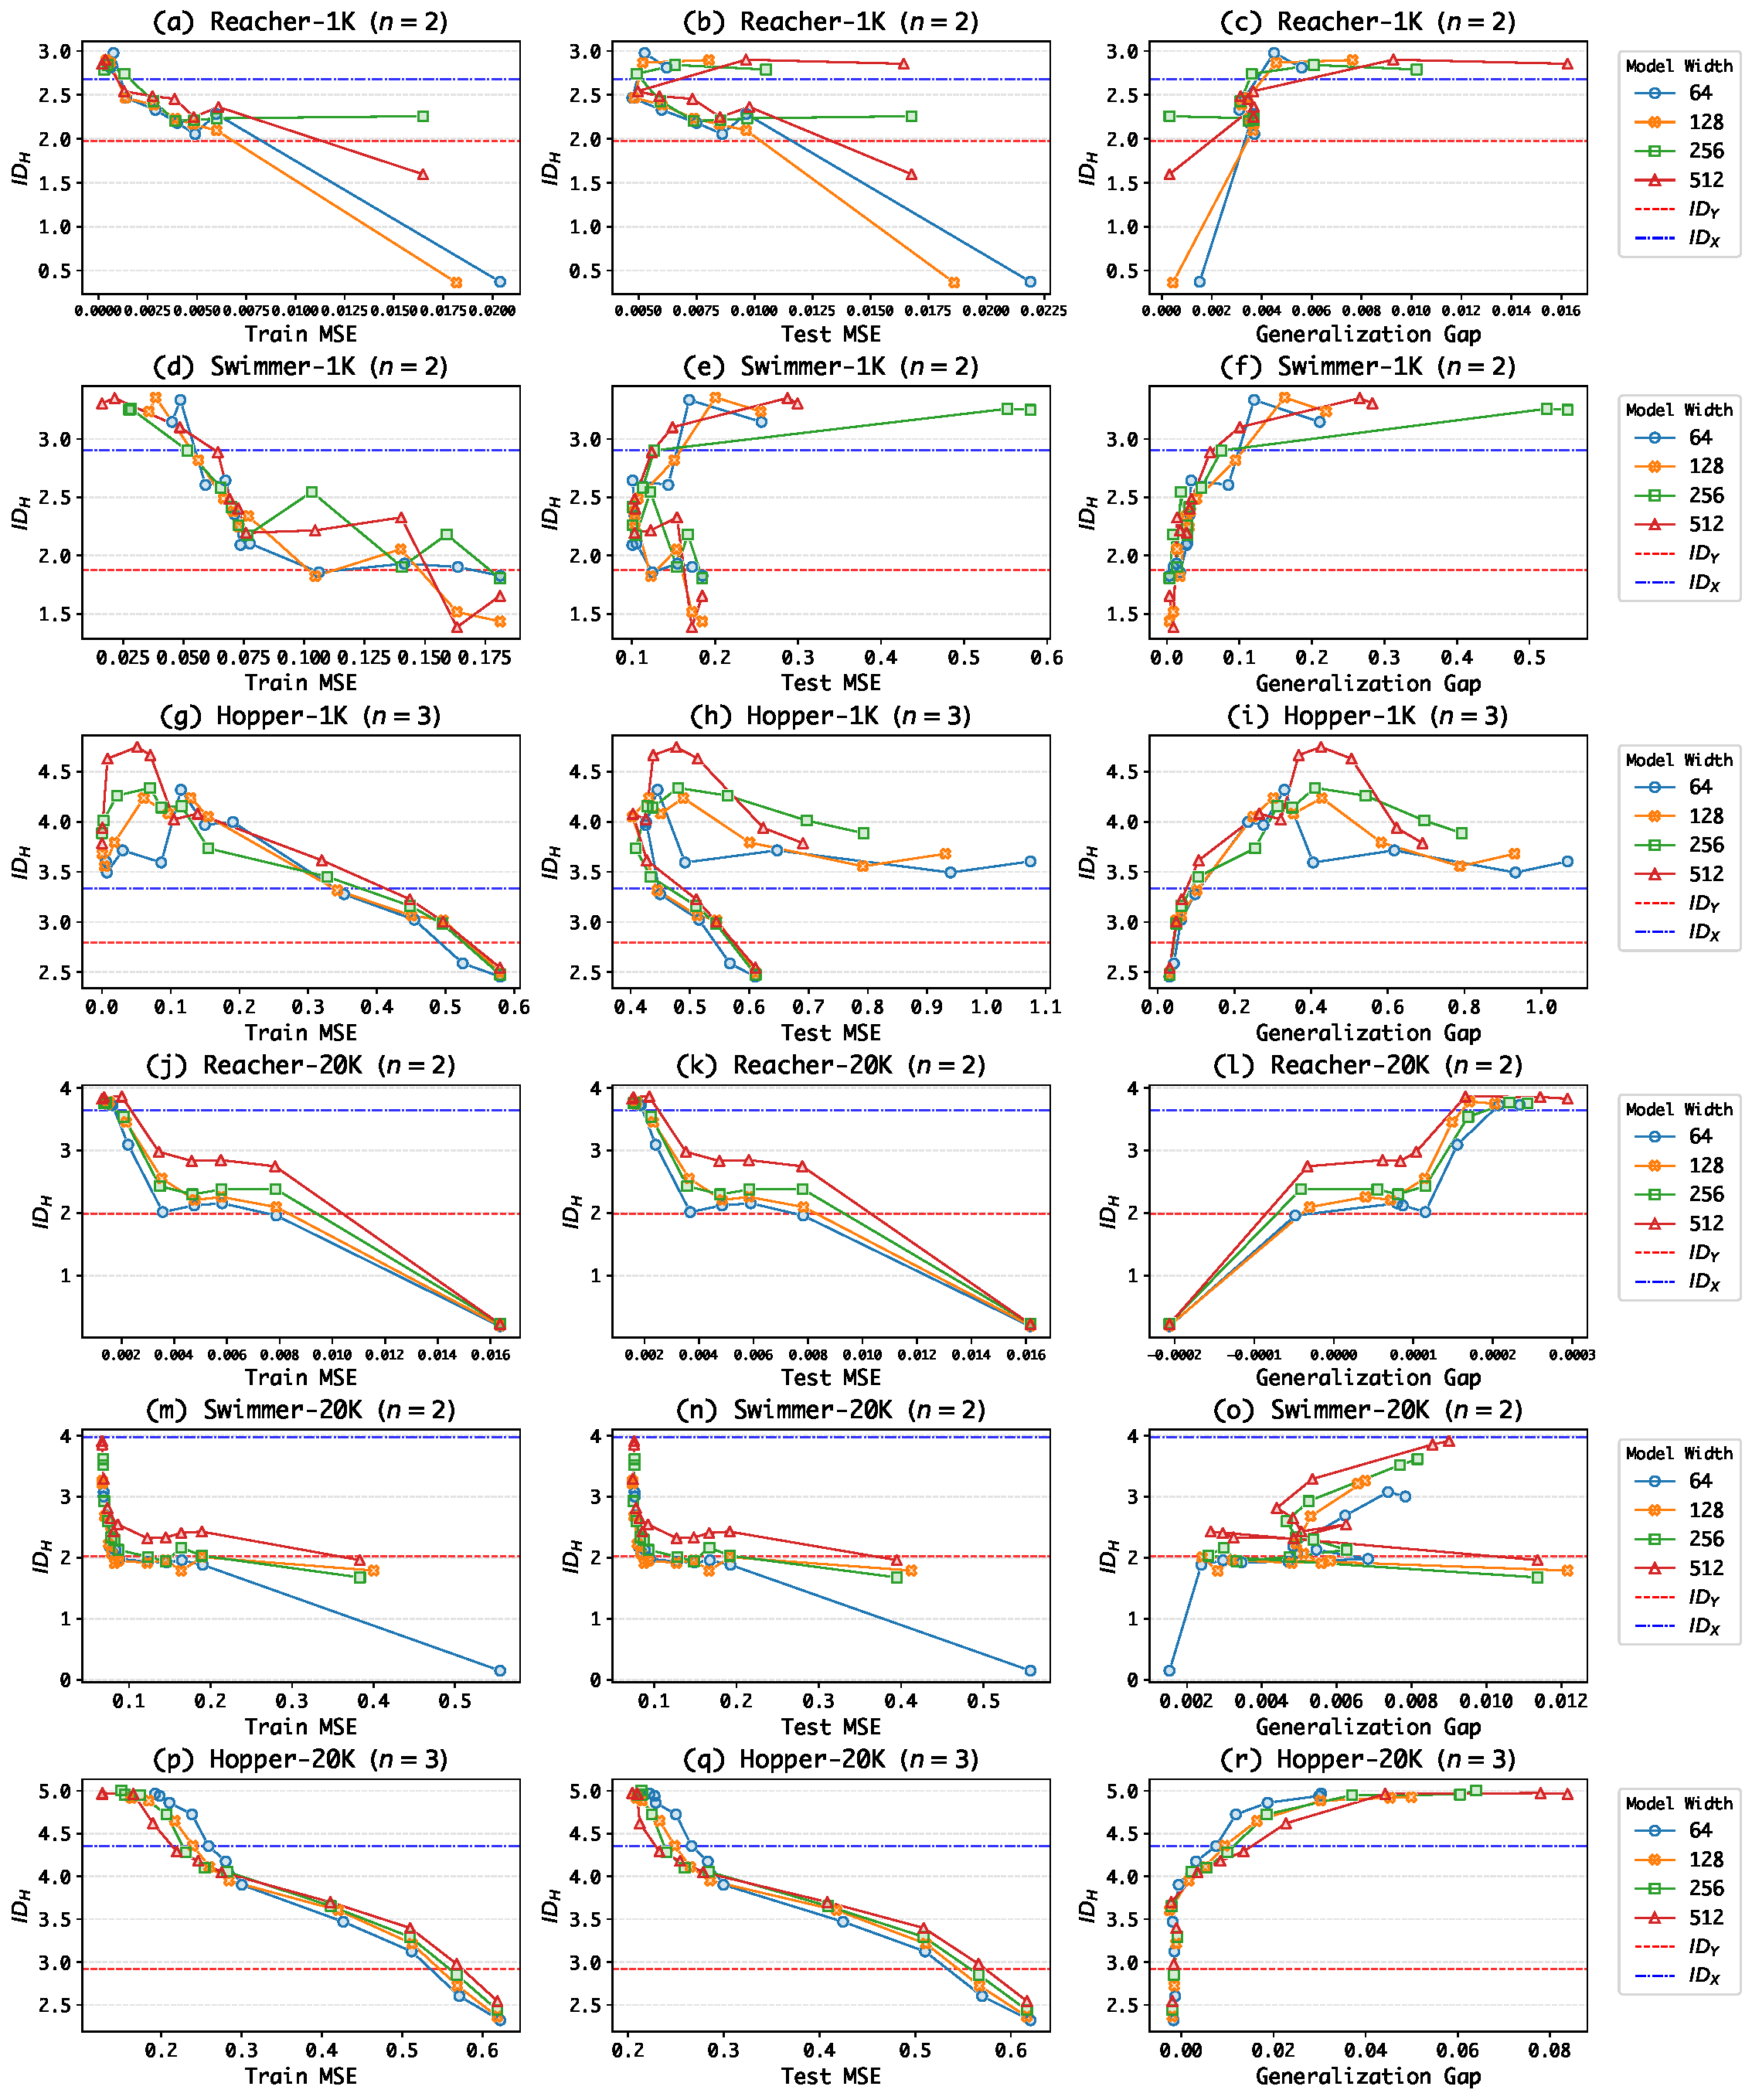
\includegraphics[width=\linewidth]{figures/Appendix/generalization_full_1.pdf}
    \caption{Generalization ability and Intrinsic Dimension for Reacher, Swimmer, and Hopper datasets.}
    \label{fig_appx:generalization_appx_2}
\end{figure}



\clearpage 
\section{How does regularization affect NRC and Intrinsic Dimension?}
\label{appx:nrc1_regularization}
\subsection{Weight Decay} \label{appx: nrc1_wd}
Weight decay is a canonical and widely adopted model regularization technique for preventing large models from overfitting to data. Real-world applications include but are not limited to (1) regularizing transformer backbones for large language models \citep{wolf-etal-2020-transformers} and robotic generalist policies \citep{chen2021decision}; (2) participating, by default, in the common Pytorch implementation of AdamW optimizer \citep{loshchilov2018adamw, pytorchAdamW} with $\texttt{weight\_decay=0.01}$; (3) improving sample efficiency of online reinforcement learning algorithms \citep{liu2021regularization, li2023efficient}; (4) and facilitating research in model plasticity in deep learning \citep{lyle2023understanding, nauman2024overestimation, ceron2024pruned}.

Figure \ref{fig_appx:nrc1_wd} investigates NRC1 for values of the weight decay parameter $\lambda_{WD}$. We see that when $\lambda_{WD}$ is zero or small, there is no neural regression collapse; but if we increase the weight decay, the NRC1 geometric structure quickly emerges during training. This matches the empirical observation in \citet{andriopoulos2024prevalence}.

\begin{figure}[htpb]
    \centering
    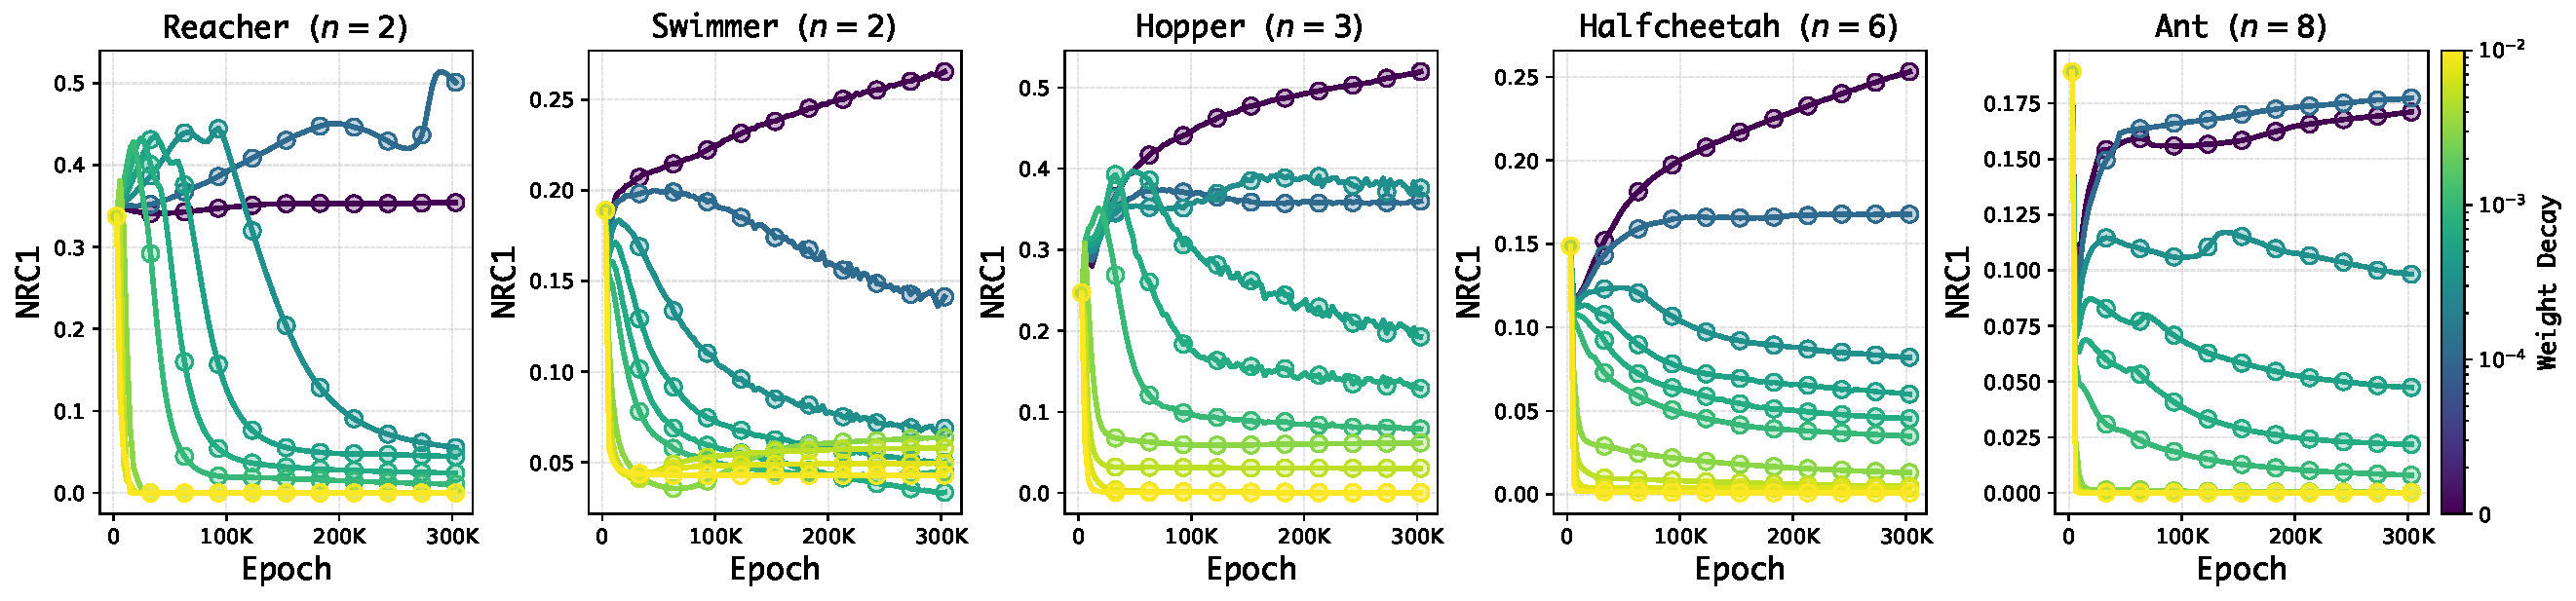
\includegraphics[width=\linewidth]{figures/Appendix/figure3_appx.pdf}
    \caption{NRC1 decreases as weight decay becomes stronger, leading to model collapse.}
    \label{fig_appx:nrc1_wd}
\end{figure}

\subsection{Dropout Regularization}
Modern implementations, across deep learning domains, continue to rely on dropout regularization \citep{srivastava14adropout} to mitigate overfitting, underscoring its persistent role in practical training, such as computer vision \citep{dosovitskiy2021vit}, NLP \citep{devlin2019bert, wolf-etal-2020-transformers}, and reinforcement learning \citep{hiraoka2022droq}. We empirically analyze how dropout regularization influences neural regression collapse by varying its strength from a large range ($\in \{0, 0.0001, 0.0005, 0.001, 0.005, 0.01, 0.05, 0.1, 0.2, 0.3, 0.4, 0.5, 0.6, 0.7, 0.8\}$). \emph{No} weight decay is applied. In this section, datasets include Hopper, Halfcheetah, and Ant with two sizes, 1K (Figure~\ref{fig:dropout_1k}) and 20K (Figure~\ref{fig:dropout_20k}). The horizontal red dashed line represents $\idy$.

Figure~\ref{fig:dropout_1k}(a) and Figure~\ref{fig:dropout_20k}(a) show the relationship between $\idh$ and NRC1. We first confirm the same conclusion as made in Section 5, despite the new regularization. $\idh$ provides a more refined geometric structure than NRC1. Collapsed models with near-zero NRC1 values have varying $\idh$ below or in the vicinity of $\idy < n$, while non-collapsed models with non-trivial NRC1 maintain their $\idh$ to be above $\idy$ and to be positively correlated with $NRC1$. Interestingly, dropout regularization differs from weight decay in that mild dropout (e.g., $\leq 0.01$) can effectively prevent models from collapse by increasing both NRC1 and $\idh$. This observation sheds light on a geometric interpretation of the effectiveness of mild dropout in reinforcement learning as proposed by \citet{hiraoka2022droq}.

Figure~\ref{fig:dropout_1k}(b) and Figure~\ref{fig:dropout_20k}(b) show the relationship between $\idh$ and test MSE. The results again verify the three regimes discussed in Section 6. For both data sizes, models over-compress features when $\idh < \idy$ and thus lead to increasing test MSE (and thus poor generalization). Then, for small datasets with 1K samples, $\idh \approx \idy$ identifies the sweet spot where test MSE tends to be the lowest and exhibits the `U-shape' plots. Note that models trained with Hopper datasets have not collapsed yet, so they only exhibit the upper part of the `U-shape'. Finally, with more samples, e.g., 20K, $\idh \gg \idy$ achieves the best generalization with under-compressed models. 

In summary, dropout regularization offers an alternative approach to adjusting the degree of model collapse, while all conclusions drawn from the main body remain intact and inclusive. In addition, mild dropout regularization is more effective than weight decay regularization in increasing NRC1 and $\idh$ metrics for the under-compressed regime.

\begin{figure}[ht]
    \centering

    \subfloat[NRC1 - $\idh$]{%
        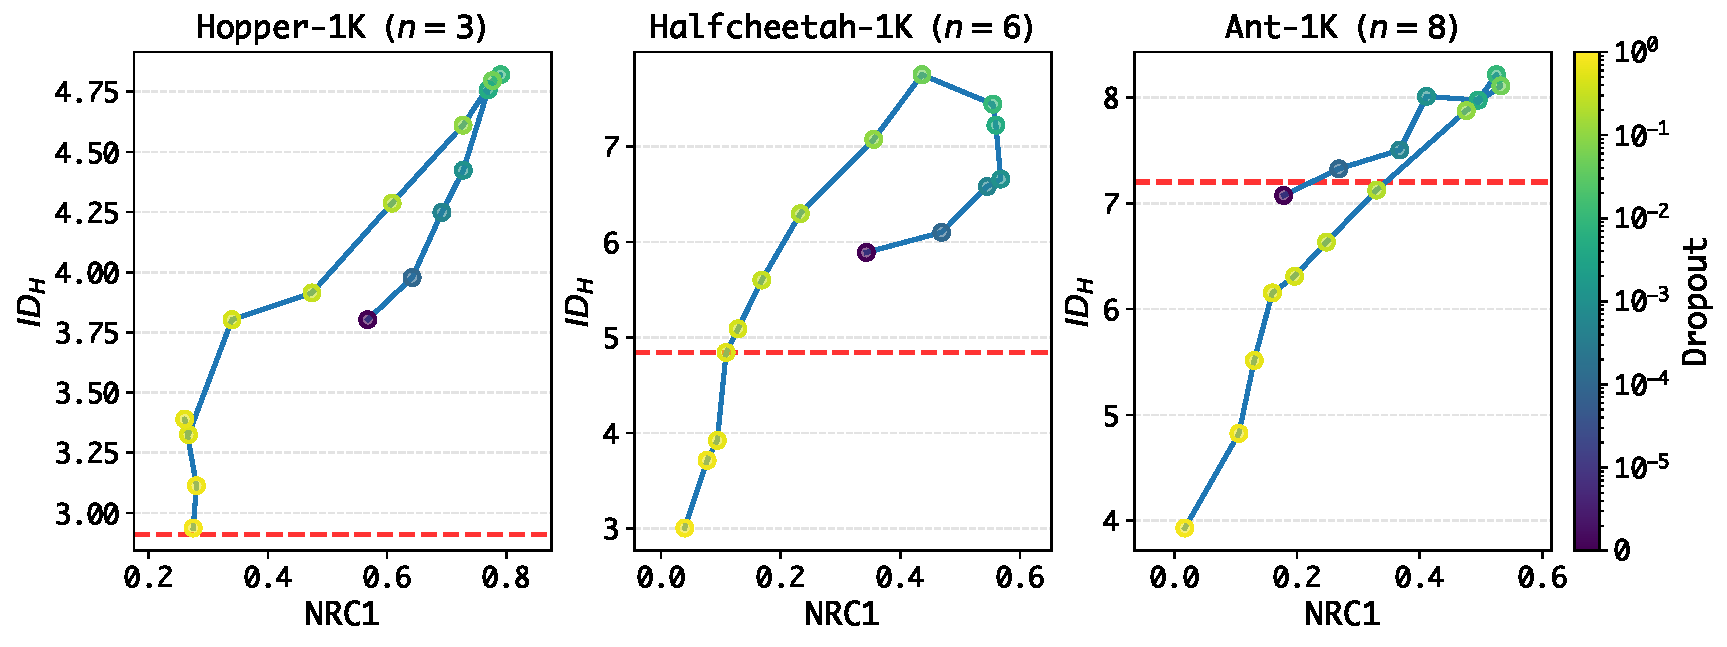
\includegraphics[width=0.65\linewidth]{figures/Rebuttal/dropout_xNRC1_yIDH_kDro_ds1K.pdf}
    }\\[1em]

    \subfloat[Test MSE - $\idh$]{%
        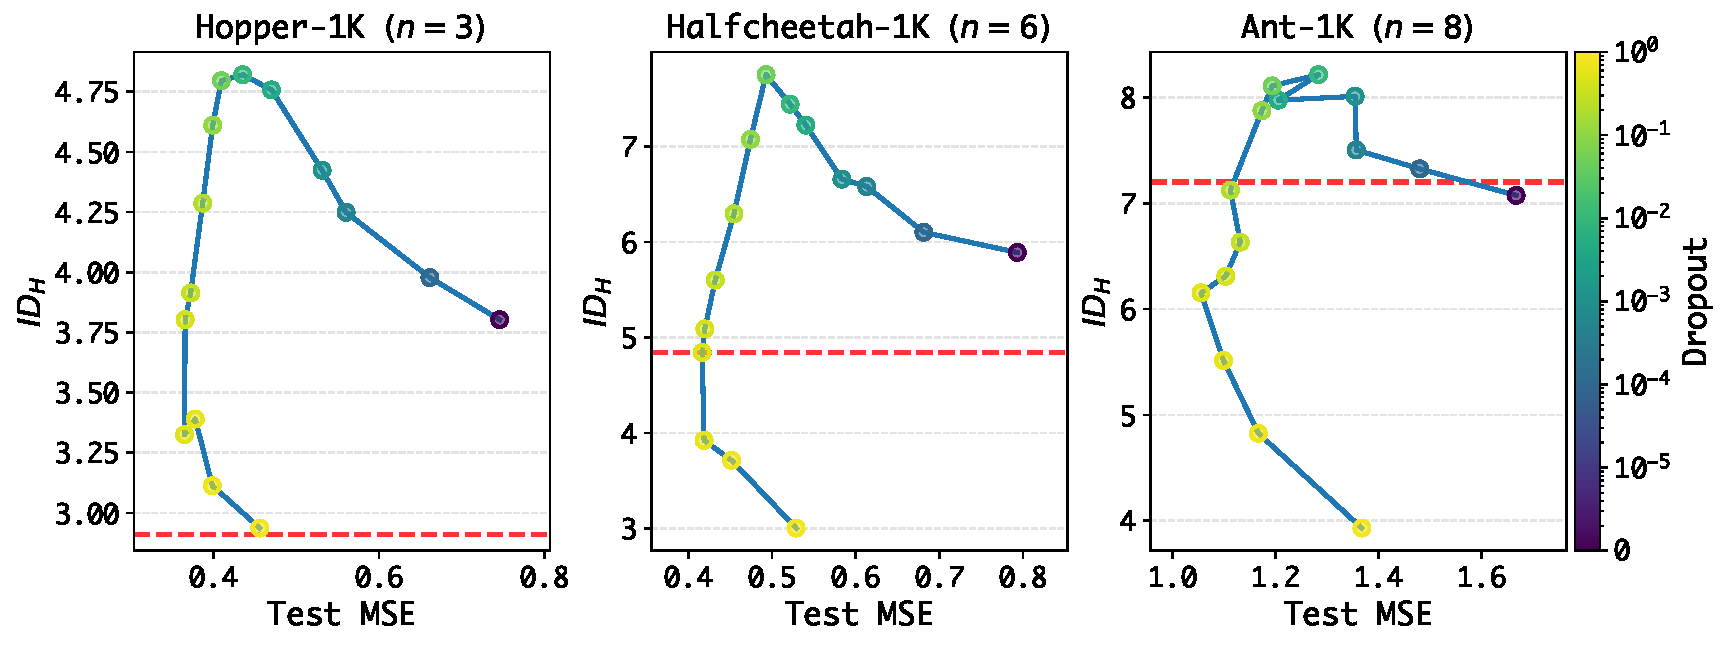
\includegraphics[width=0.65\linewidth]{figures/Rebuttal/dropout_xMSE_yIDH_kDro_ds1K.pdf}
    }

    \caption{Relationship between $\idh$ and NRC1 and Test MSE for Hopper-1K, Halfcheetah-1K, and Ant-1K datasets, when applying model dropout regularization. The horizontal red dashed line represents $\idy$.}
    \label{fig:dropout_1k}
\end{figure}

\begin{figure}[ht]
    \centering

    \subfloat[NRC1 - $\idh$]{%
        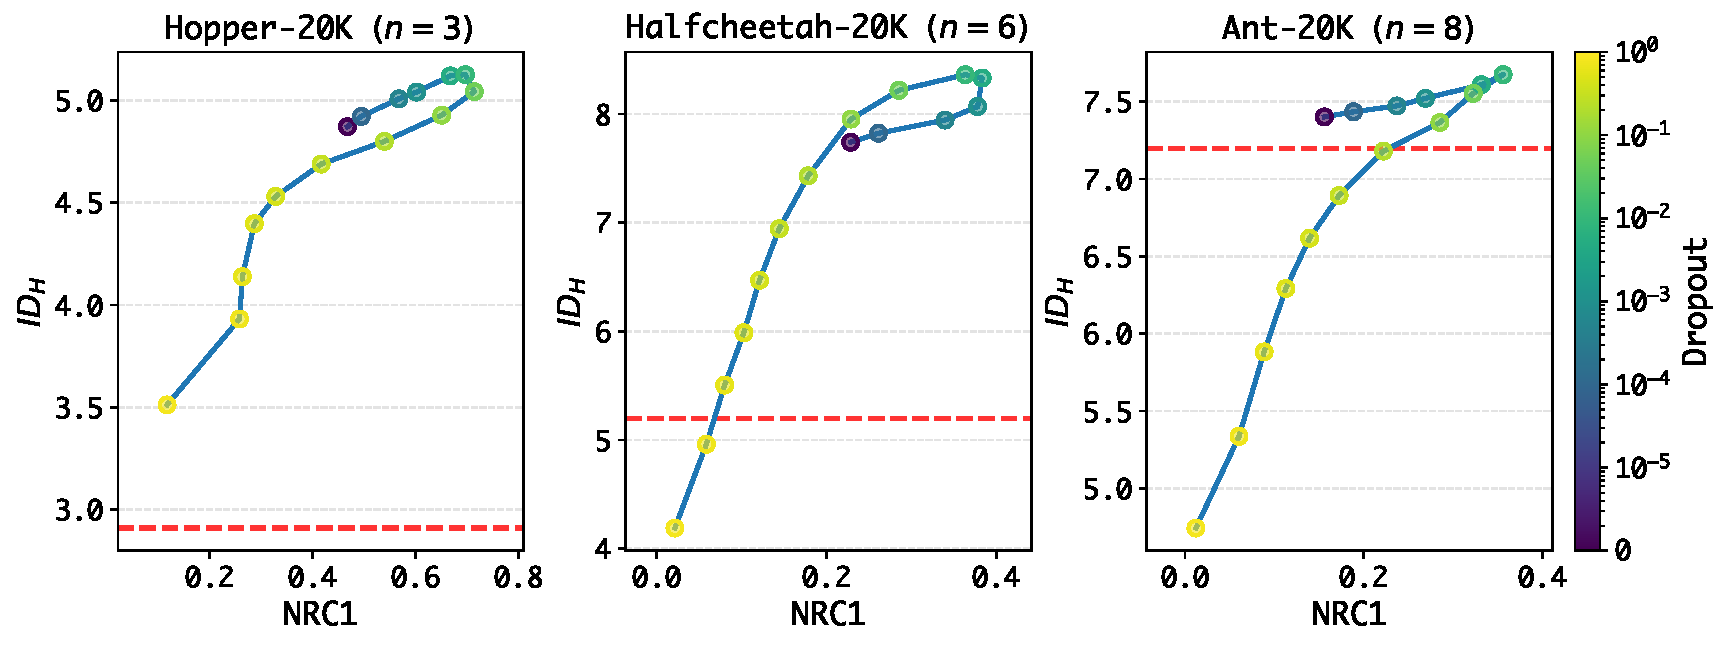
\includegraphics[width=0.65\linewidth]{figures/Rebuttal/dropout_xNRC1_yIDH_kDro_ds20K.pdf}
    }\\[1em]

    \subfloat[Test MSE - $\idh$]{%
        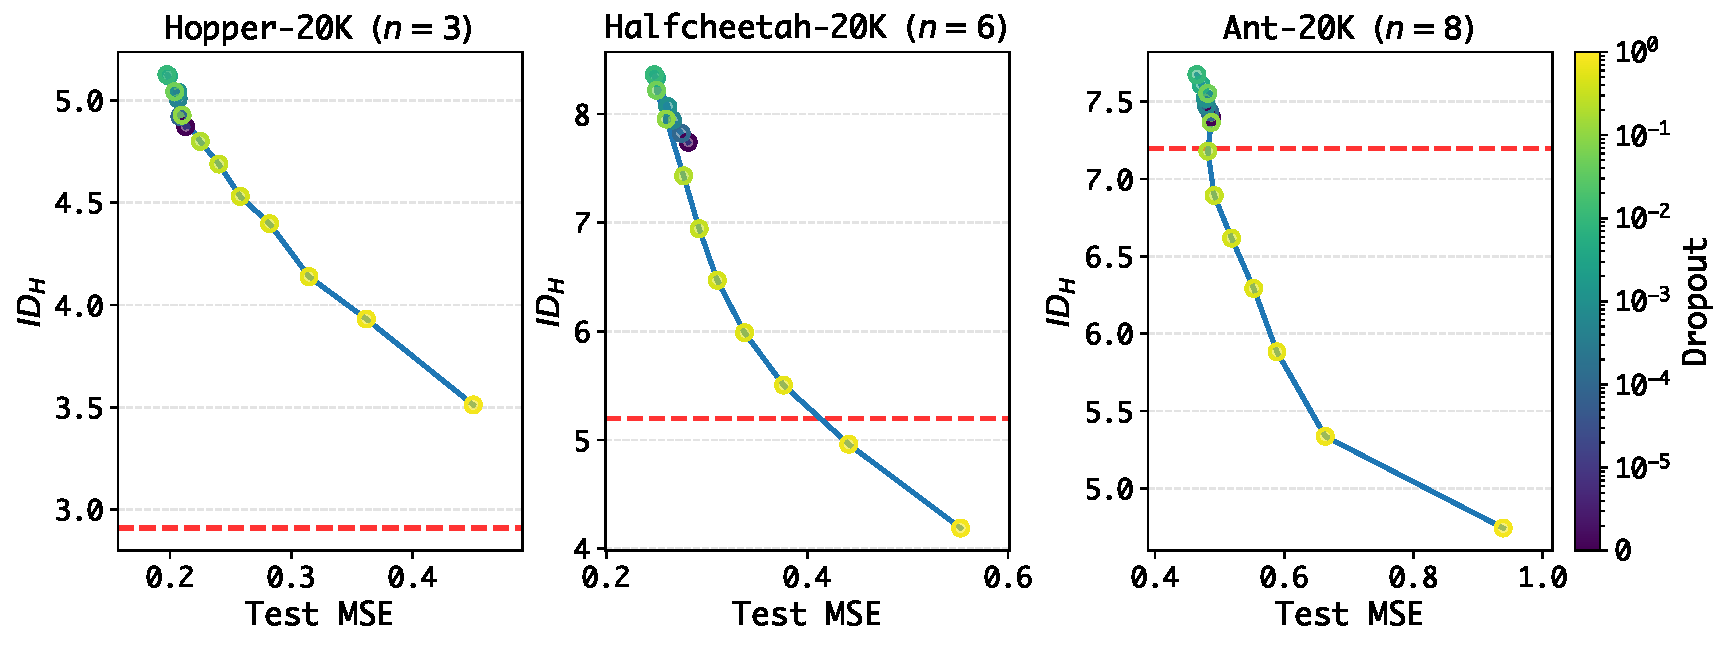
\includegraphics[width=0.65\linewidth]{figures/Rebuttal/dropout_xMSE_yIDH_kDro_ds20K.pdf}
    }

    \caption{Varying model dropout regularization, relationship between $\idh$ and NRC1 and Test MSE for Hopper-20K, Halfcheetah-20K, and Ant-20K datasets. The horizontal red dashed line represents $\idy$.}
    \label{fig:dropout_20k}
\end{figure}


\subsection{Model Depth}
With mild weight decay regularization, we find that increasing model depth leads to smaller NRC1 and $\idh$ and thus to more collapsed features. In Figure~\ref{fig:model_depth}, we examine the relationship between $\idh$ and NRC1 for Hopper-20K and Halfcheetah-20K datasets. We fix the model width to be 256 and vary the model depth ($\in \{2, 3, 4, 5\}$). For each model depth, we show five mild weight decay values: 0.0001, 0.0003, 0.0005, 0.0007, 0.001. The figure shows that increasing model depth gradually pushes points to the region on the bottom left, where both NRC1 and $\idh$ are small. For example, Halfcheetah-20K with a depth of 5 can result in collapsed models with $\idh < \idy$. 


\begin{figure}[h]
    \centering
    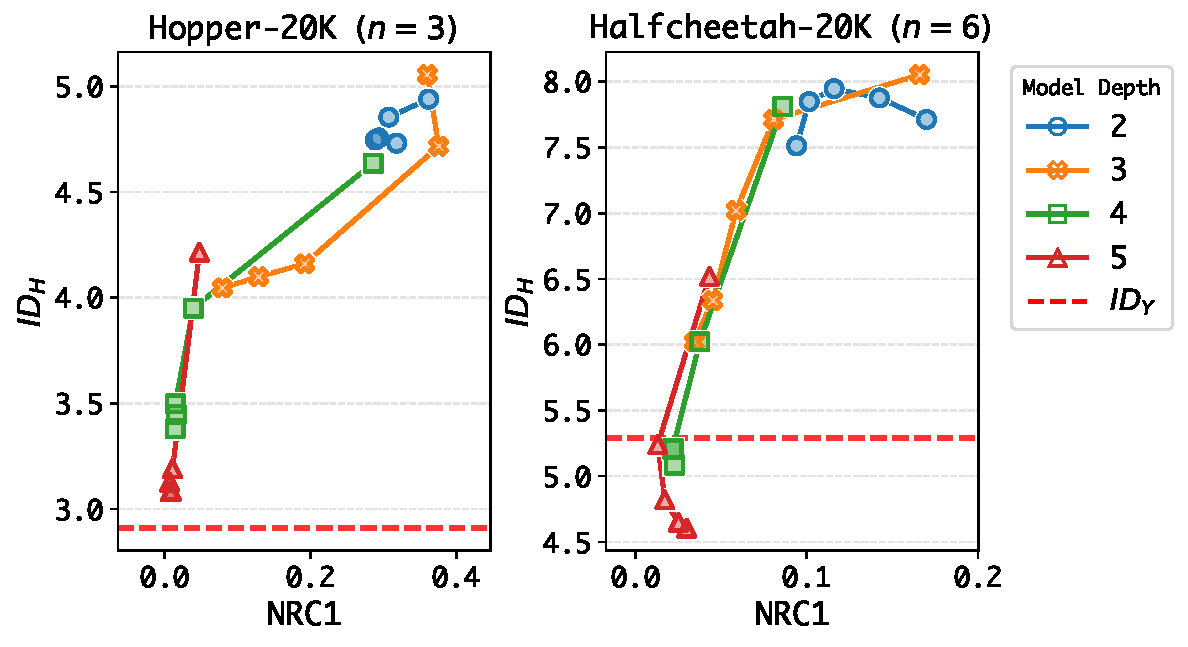
\includegraphics[width=0.6\linewidth]{figures/Rebuttal/depth_xNRC1_yIDH_kDepth.pdf}
    \caption{Relationship between $\idh$ and NRC1 for Hopper-20K and Halfcheetah-20K datasets, when varying model depth. All models have a hidden size of 256. The horizontal red dashed line represents $\idy$.}
    \label{fig:model_depth}
\end{figure}


\section{Empirical Analysis on More Challenging Tasks}
\label{appx:more_tasks}
We extend our empirical analysis to more challenging tasks with varying data sizes, increased intrinsic dimensions, and visual inputs.

\begin{table}[h!]

\caption{Overview of additional datasets employed in this section.}
\begin{center}

\scalebox{0.75}{
\begin{tabular}{ccccccc}
\toprule
\textbf{Dataset} & \textbf{Data Size} & \textbf{Input Type} &\textbf{Input Dim ($D$)} & \textbf{Input ID ($\idx$)} & \textbf{Target Dim} ($n$) & \textbf{Target ID ($\idy$)}\\
\midrule
Humanoid & 500,000 & raw state & 348 & 11.02 & 17 & 9.85\\

Relocate & 500,000 & raw state & 39 & 6.90 & 30 & 19.82 \\

\midrule
Cheetah\_run & 80,000 & RGB image & $84\times84\times9$\footnotemark & 8.96 & 6 & 6.00\\

Humanoid\_walk & 100,000 & RGB image & $84\times84\times9$ & 9.41 & 21 & 14.84\\
    
\bottomrule
\end{tabular}
}

\end{center}
\label{table:dataset_appx}
\end{table} 

\footnotetext{Frame stack is commonly applied for visual control tasks. A single observation is of shape $84\times84\times3$. A frame stack of 3 is used in our experiments, resulting in visual inputs of dimension $84\times84\times9$.}

\paragraph{Humanoid (MuJoCo locomotion)}
The Humanoid dataset \citep{minari} is generated from the MuJoCo physics simulator, introduced in the main body and Appendix~\ref{appx: mujoco}. Each state consists of high-dimensional proprioceptive information, and the corresponding targets are the expert control torques applied at each joint. The goal is to enable the humanoid to run forward stably while maintaining balance, which is substantially more difficult than all previously considered MuJoCo tasks due to its high degrees of freedom and complex contact dynamics. Among all MuJoCo environments, Humanoid is widely regarded as the most challenging.

\paragraph{Relocate (Adroit manipulation)}
The Relocate dataset \citep{fu2020d4rl} comes from the Adroit suite \citep{rajeswaran18adroit} of dexterous manipulation tasks. Adroit uses a simulated 24 degrees of freedom (24-DoF) robotic hand, combined with an arm of up to 6-DoF, with rich contact and articulation dynamics. In the Relocate task, the state includes joint positions, velocities, hand pose information, and kinematic information about the ball and target. The action corresponds to the joint torques for the 24 actuators and to the arm movement. The objective is to grasp a small object and relocate it to a specified target position. It is a long-horizon manipulation task requiring precise coordination and contact control. Among the four Adroit tasks in the D4RL benchmark \citep{fu2020d4rl}, Relocate is widely considered the most difficult due to its combination of dexterity, precision, and exploration complexity.

\paragraph{Cheetah\_run \& Humanoid\_walk (Visual continuous control)}
The Cheetah\_run and Humanoid\_walk datasets \citep{lu2023vd4rl} are visual control benchmarks constructed from demonstrations generated in the DeepMind Control Suite \citep{tassa2018deepmindcontrolsuite}. Inputs consist of raw image observations (e.g., 84×84x3 RGB frames), and targets correspond to the continuous control commands. In this section, the Cheetah\_run dataset consists of expert demonstrations, as is the case for all previous datasets, while the Humanoid\_run dataset contains some noisy suboptimal behavior in addition to the expert demonstrations (`medium-expert dataset'). This adds difficulty in extracting a good policy by imitating the dataset's behavior. We use a CNN image encoder (consisting of 4 \texttt{conv2d} layers and ReLU activation), followed by a 3-layer MLP policy network.

Visual control is particularly interesting and challenging because each frame provides only partial information about the system state, effectively forming a Partially Observed Markov Decision Process (POMDP) \citep{yarats2022drq_v2}. As a result, the model must infer underlying transition dynamics and identify salient visual features directly from high-dimensional pixel inputs. Within the visual D4RL tasks \citep{lu2023vd4rl}, Humanoid\_walk is the most challenging due to the humanoid’s instability and high-dimensional dynamics, whereas Cheetah\_run is comparatively easier but still nontrivial.

\begin{figure}[ht]
    \centering

    \subfloat[NRC1 - $\idh$]{%
        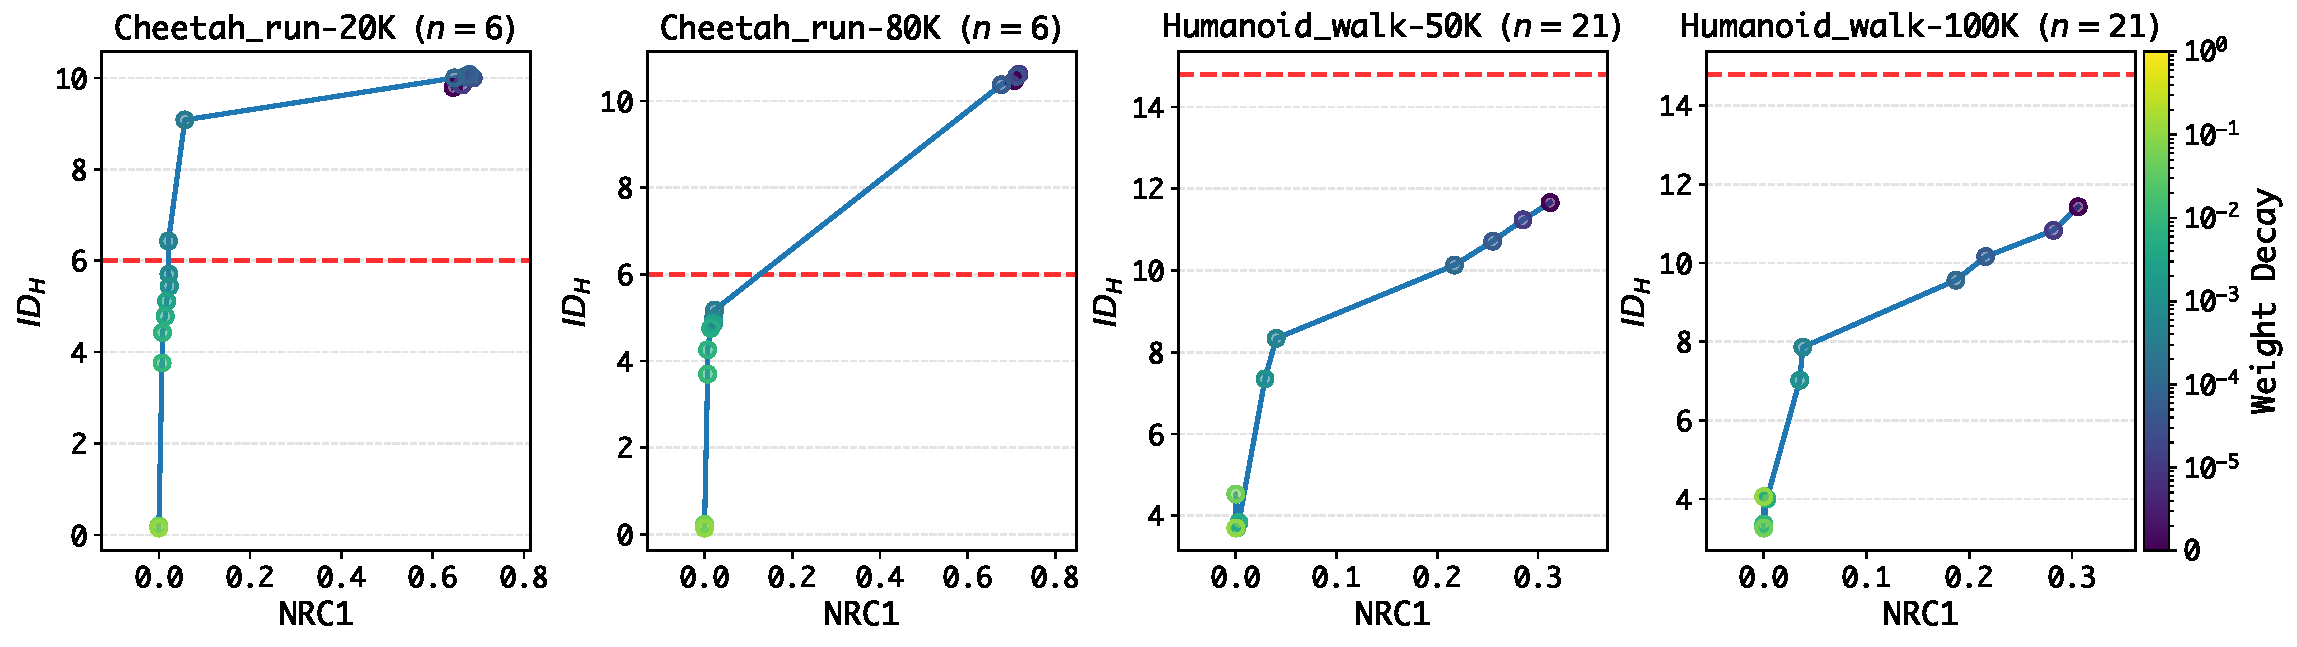
\includegraphics[width=0.90\linewidth]{figures/Appendix/vd4rl_nrc1.pdf}
    }\\[1em]

    \subfloat[Test MSE - $\idh$]{%
        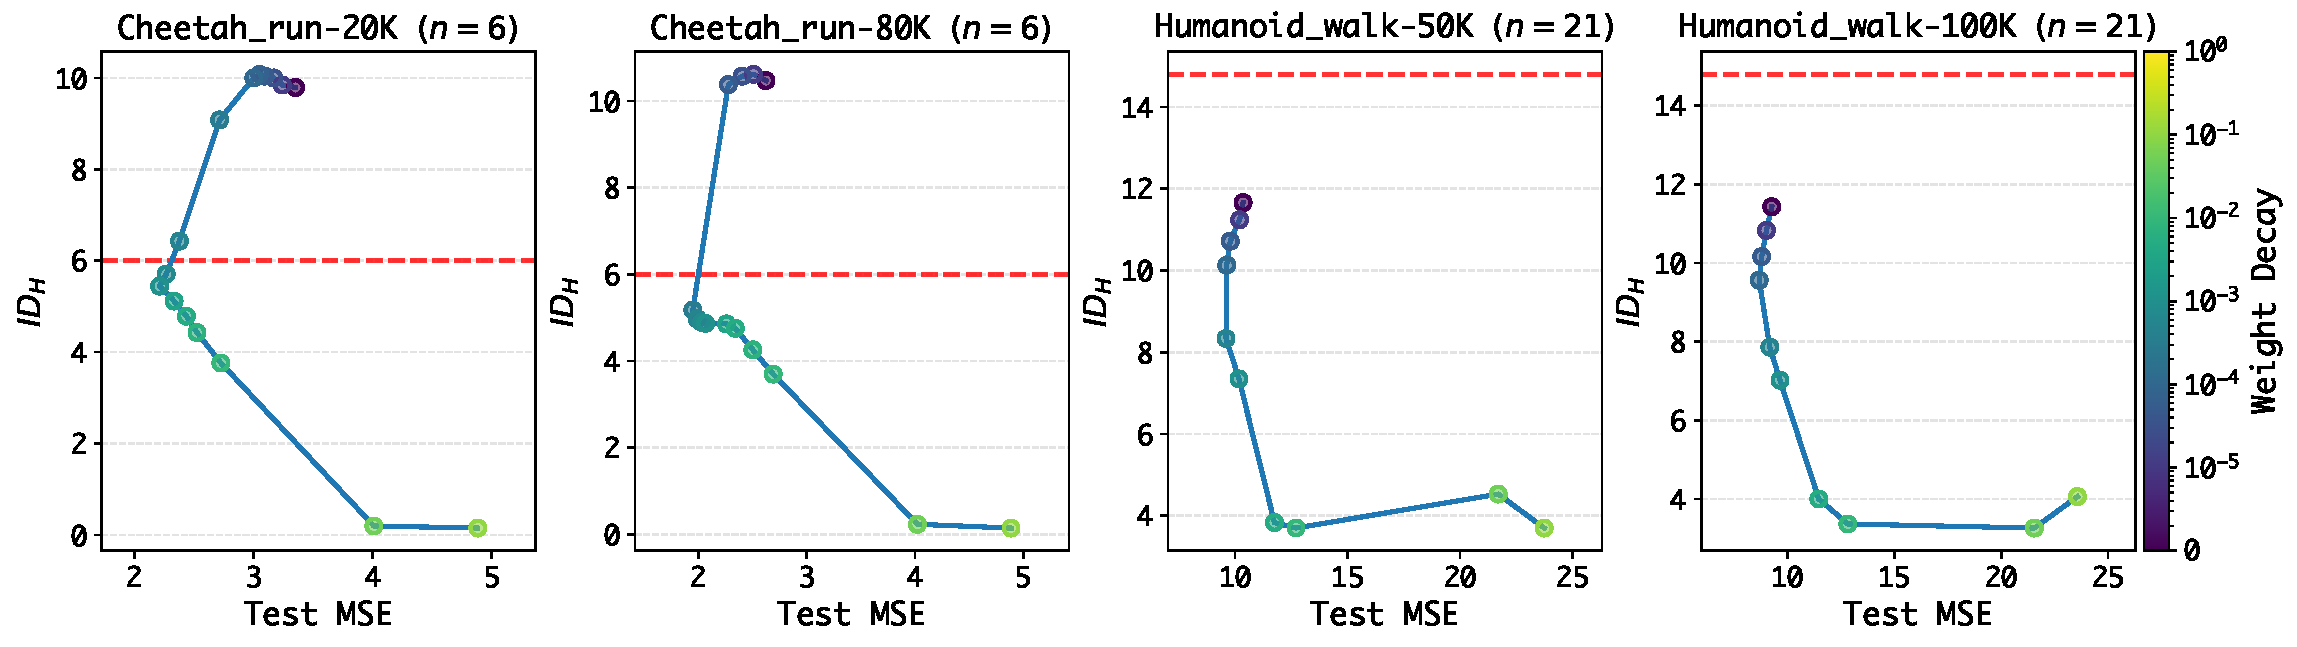
\includegraphics[width=0.90\linewidth]{figures/Appendix/vd4rl_mse.pdf}
    }

    \caption{Relationship between $\idh$ and NRC1 and Test MSE for Cheetah\_run-20K, Cheetah\_run-80K, Humanoid\_walk-50K and Humanoid\_walk-100K. The horizontal red dashed line represents $\idy$.}
    \label{fig:vd4rl_main}
\end{figure}


\subsection{Visual Control Tasks} 
Figure~\ref{fig:vd4rl_main}(a) shows the relationship between $\idh$ and NRC1 for the visual control datasets with varying sizes. Consistent with the conclusions in Section 5, $\idh$ provides a more refined geometric structure than NRC1. Collapsed models with small NRC1 values have varying $\idh$ below or in the vicinity of $\idy < n$, while non-collapsed models with non-trivial NRC1 maintain their $\idh$ to be above $\idy$ and to be positively correlated with NRC1. Notably, for the most challenging Humanoid\_walk task, which has a substantially higher $\idy$ due to its complex high-dimensional dynamics, models trained with \emph{zero} weight decay initially exhibit neural regression collapse with $\idh < \idy$. This explains the extremely large test MSE observed for Humanoid\_walk in Figure~\ref{fig:vd4rl_main}(b) and its negative correlation with $\idh$, which matches the over-compressed regime ($\idh < \idy$) summarized in Table~\ref{table:gen}. In comparison, the two Cheetah\_run datasets exhibit the `U-shape' in the relationship between $\idh$ and test MSE. This emphasizes the sweet spot with $\idh \approx \idy$, which approaches the lowest test MSE in noisy and challenging tasks.

\subsection{Relocate \& Humanoid}
\paragraph{Humanoid} In Figure~\ref{fig:size_humanoid}, we show `NRC1 - $\idh$' and `Test MSE - $\idh$' plots for Humanoid datasets with varying sizes. In Figure~\ref{fig:size_humanoid}(a), we observe that $\idh$ provides a more refined geometric structure than NRC1. Collapsed models with near-zero NRC1 values have varying $\idh$ below or in the vicinity of $\idy < n$, while non-collapsed models with non-trivial NRC1 maintain their $\idh$ to be above $\idy$ and to be positively correlated with NRC1. Then, Figure~\ref{fig:size_humanoid}(b) again verifies the three regimes discussed in Section 6. For all data sizes, models over-compress features when $\idh < \idy$ and thus lead to increasing test MSE (and thus poor generalization). Then, for small datasets with 1-50K samples, $\idh \approx \idy$ identifies the sweet spot where test MSE tends to be the lowest and exhibits the `U-shape' plots. Finally, with more samples, e.g., 100-500K, $\idh > \idy$ achieves the best generalization with under-compressed models. 

\paragraph{Relocate} 
For the Relocate task with varying data sizes, which have the highest $\idy$ due to its complex task dynamics, models trained with \emph{zero} weight decay initially exhibit a severe collapse with both $\text{NRC1} \approx 0$ and $\idh \ll \idy$. Unsurprisingly, Test MSE remains large for all data sizes and decay values, and it also negatively correlates with $\idh$, uncovering the over-compressed regime.

\begin{figure}[ht]
    \centering

    \subfloat[NRC1 - $\idh$]{%
        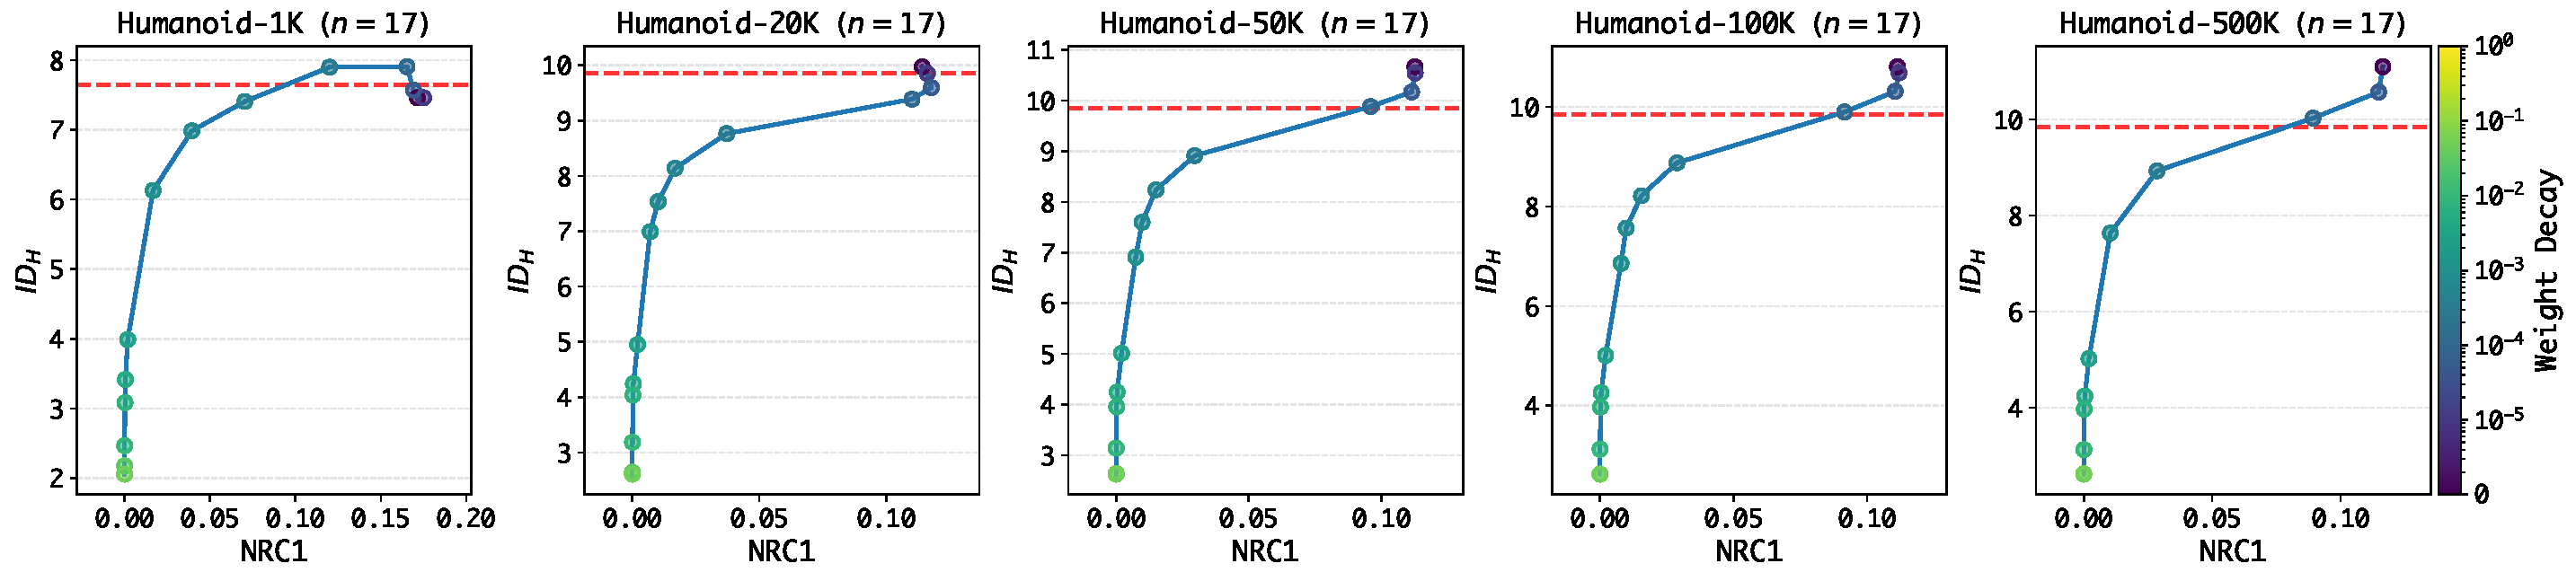
\includegraphics[width=1\linewidth]{figures/Rebuttal/size_xNRC1_yIDH_kWD_humanoid.pdf}
    }\\[1em]

    \subfloat[Test MSE - $\idh$]{%
        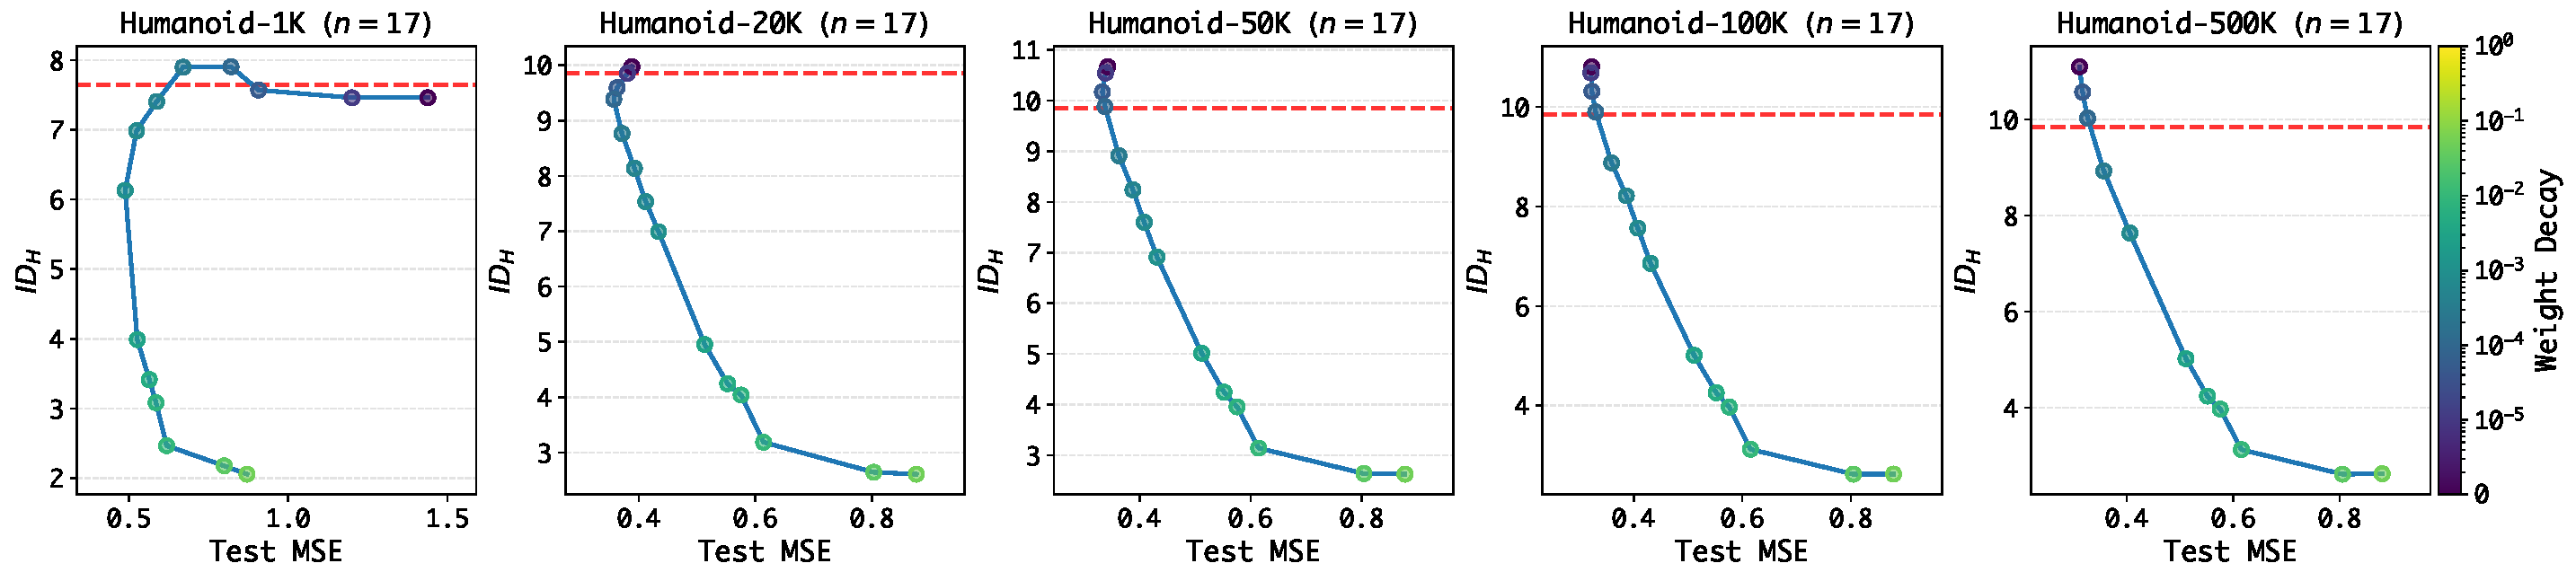
\includegraphics[width=1\linewidth]{figures/Rebuttal/size_xMSE_yIDH_kWD_humanoid.pdf}
    }

    \caption{Relationship between $\idh$ and NRC1 and Test MSE, for Humanoid locomotion task, when varying data size ($\in \{\text{1K}, \text{20K}, \text{50K}, \text{100K}, \text{500K}\}$). The red dashed line represents $\idy$.}
    \label{fig:size_humanoid}
\end{figure}

\begin{figure}[ht]
    \centering

    \subfloat[NRC1 - $\idh$]{%
        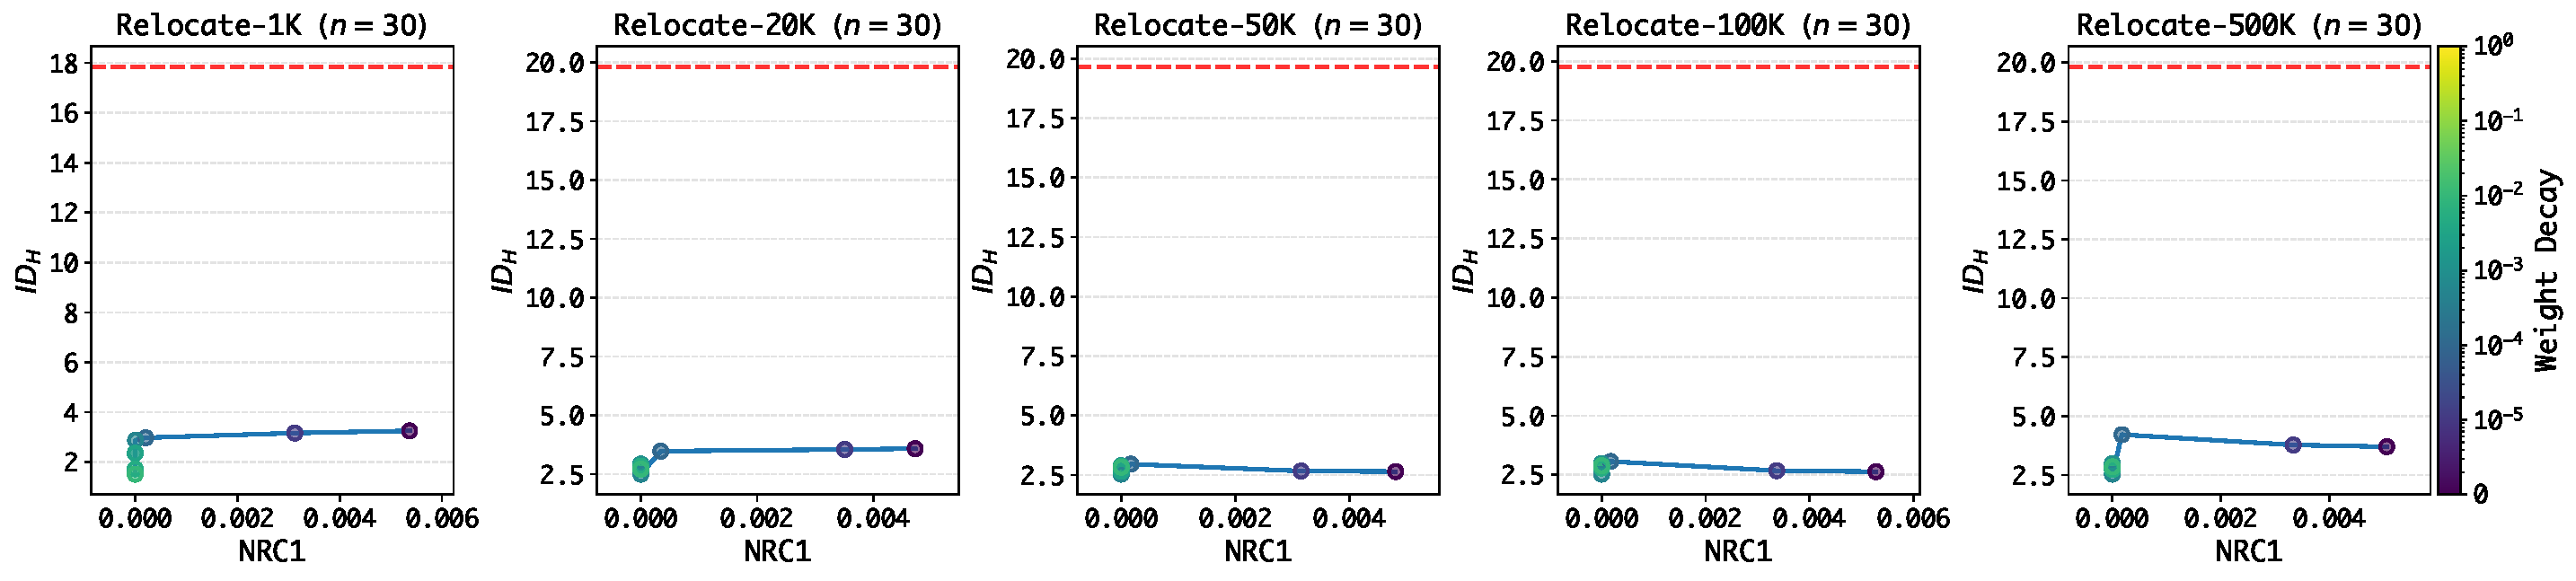
\includegraphics[width=1\linewidth]{figures/Rebuttal/size_xNRC1_yIDH_kWD_relocate.pdf}
    }\\[1em]

    \subfloat[Test MSE - $\idh$]{%
        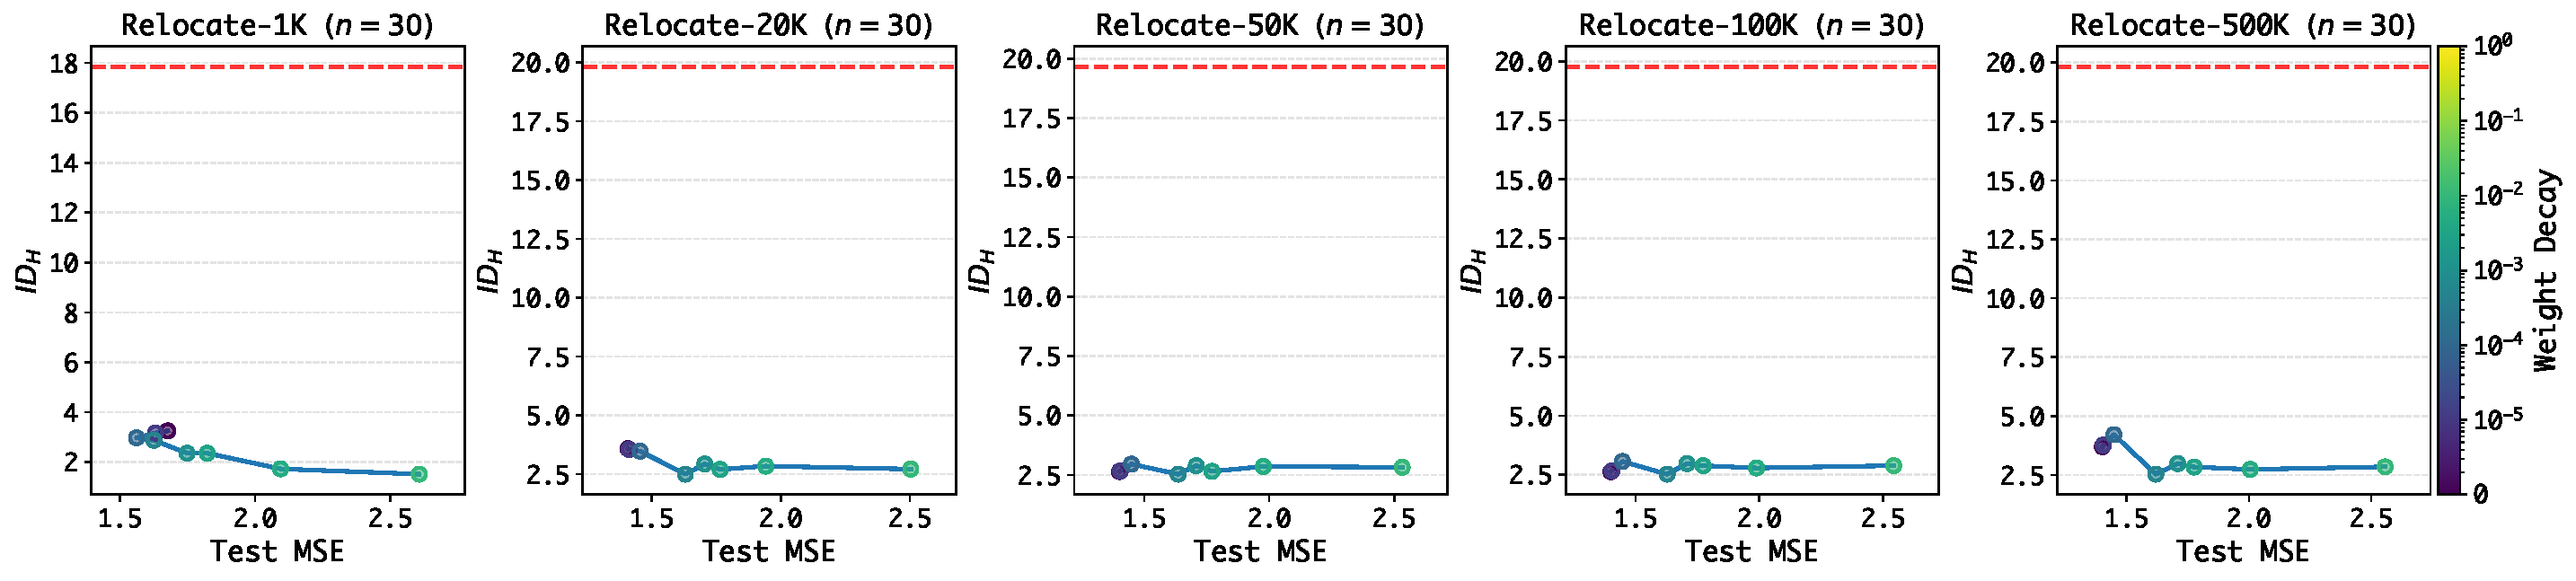
\includegraphics[width=1\linewidth]{figures/Rebuttal/size_xMSE_yIDH_kWD_relocate.pdf}
    }

    \caption{Relationship between $\idh$ and NRC1 and Test MSE, for Relocate manipulation task, when varying data size ($\in \{\text{1K}, \text{20K}, \text{50K}, \text{100K}, \text{500K}\}$). The red dashed line represents $\idy$.}
    \label{fig:size_relocate}
\end{figure}





\clearpage
\section{Mathematical Analysis of Regression Collapse}
\label{appx:mathematical_analysis}

\subsection{Why Weight Decay Leads to Collapse: Analysis via the Unconstrained Feature Model}
\label{appx:ufm_collapse}

In this section, we provide a theoretical explanation for why weight decay causes neural regression collapse through the lens of the Unconstrained Feature Model (UFM). The UFM is a simplified mathematical abstraction that does not capture all aspects of practical neural networks, but provides insight into the geometric mechanisms by which regularization constrains learned representations.

The UFM abstracts the neural regression problem by treating the feature extractor $h_\theta(\cdot)$ as producing arbitrary feature vectors $\mathbf{h}_i \in \mathbb{R}^d$ for each input $\mathbf{x}_i$, collected into a feature matrix $H \in \mathbb{R}^{d \times M}$. The final prediction is obtained via a linear map $W \in \mathbb{R}^{n \times d}$ and bias $\mathbf{b} \in \mathbb{R}^n$, giving predictions $\hat{Y} = WH + \mathbf{b} \mathbf{1}^\top$. The UFM objective is:
\begin{equation}
\min_{W, H, \mathbf{b}} \frac{1}{2M} \|WH + \mathbf{b}\mathbf{1}^\top - Y\|_F^2 + \frac{\lambda_W}{2}\|W\|_F^2 + \frac{\lambda_H}{2}\|H\|_F^2
\end{equation}
The model is ``unconstrained'' because $H$ can be any matrix in $\mathbb{R}^{d \times M}$, unlike in actual neural networks, where $H$ is constrained by the input data and network architecture. In the UFM, we typically have $d \gg n$, mirroring the overparameterized regime where feature dimension greatly exceeds target dimension.

The optimal bias is $\mathbf{b}^* = \bar{\mathbf{y}}$ where $\bar{\mathbf{y}} = \frac{1}{M}\sum_{i=1}^M \mathbf{y}_i$. Defining the centered target matrix $\tilde{Y} = Y - \bar{\mathbf{y}}\mathbf{1}^\top \in \mathbb{R}^{n \times M}$, the problem reduces to:
\begin{equation}
\min_{W, H} \frac{1}{2M} \|WH - \tilde{Y}\|_F^2 + \frac{\lambda_W}{2}\|W\|_F^2 + \frac{\lambda_H}{2}\|H\|_F^2
\label{eq:ufm_centered}
\end{equation}
We denote the empirical covariance by $\Sigma = \frac{1}{M}\tilde{Y}\tilde{Y}^\top \in \mathbb{R}^{n \times n}$, and assume $\Sigma$ is full rank with eigenvalues $\lambda_1 \geq \lambda_2 \geq \cdots \geq \lambda_n > 0$. A key quantity is $c = \lambda_W \lambda_H$.

We first restate the characterization of global minimizers when regularization is present, adapted from Theorem 4.1 of \citet{andriopoulos2024prevalence}. We focus on the regime where $c < \lambda_n$ since we are interested in the limiting behavior when $\lambda_H \to 0$ and $\lambda_W \to 0$.

\begin{theorem}[Regularized UFM Solution, adapted from \citet{andriopoulos2024prevalence}]
\label{thm:ufm_regularized}
Suppose $0 < c < \lambda_n$. Define $A = \Sigma^{1/2} - \sqrt{c} I_n$. Then any global minimizer $(W_\lambda, H_\lambda)$ of \eqref{eq:ufm_centered} can be expressed as:
\begin{align}
W_\lambda &= \left(\frac{\lambda_H}{\lambda_W}\right)^{1/4} A^{1/2} R \label{eq:w_lambda}\\
H_\lambda &= \left(\frac{\lambda_W}{\lambda_H}\right)^{1/4} R^\top A^{1/2} (\Sigma^{1/2})^{-1} \tilde{Y} \label{eq:h_lambda}
\end{align}
where $R \in \mathbb{R}^{n \times d}$ is any matrix satisfying $RR^\top = I_n$.
\end{theorem}

\begin{proof}
This follows from Theorem 4.1 of \citet{andriopoulos2024prevalence} with $c < \lambda_n$ implying $j^* = n$.
\end{proof}

The regularized solution has a specific dimensional structure. Since $A^{1/2}(\Sigma^{1/2})^{-1}\tilde{Y} \in \mathbb{R}^{n \times M}$ and $R^\top \in \mathbb{R}^{d \times n}$, the matrix $H_\lambda \in \mathbb{R}^{d \times M}$ has columns lying in the column space of $R^\top$, which is at most $n$-dimensional. Even though $H_\lambda$ lives in a $d$-dimensional ambient space with $d \gg n$, its columns are confined to an $n$-dimensional subspace.

When regularization is absent, the problem has infinitely many global minimizers, characterized by the following theorem from \citet{andriopoulos2024prevalence}.

\begin{theorem}[Unregularized UFM Solutions, from \citet{andriopoulos2024prevalence}]
\label{thm:ufm_unregularized}
When $\lambda_W = \lambda_H = 0$, a pair $(W, H)$ is a global minimizer of \eqref{eq:ufm_centered} if and only if $WH = \tilde{Y}$ and $W$ has full row rank. For any such $W$, the corresponding global minimizers in $H$ are:
\begin{equation}
H_{\text{unreg}} = W^\dagger \tilde{Y} + (I_d - W^\dagger W)Z
\label{eq:h_unreg}
\end{equation}
where $W^\dagger$ is the Moore--Penrose pseudoinverse and $Z \in \mathbb{R}^{d \times M}$ is arbitrary.
\end{theorem}

\begin{proof}
See Theorem 4.3 of \citet{andriopoulos2024prevalence}.
\end{proof}

The structure in \eqref{eq:h_unreg} decomposes solutions into two orthogonal components: $W^\dagger \tilde{Y}$ lies in the row space of $W$ (dimension at most $n$), while $(I_d - W^\dagger W)Z$ lies in the null space of $W$ (dimension exactly $d - n$). The Frobenius norm satisfies $\|H_{\text{unreg}}\|_F^2 = \|W^\dagger \tilde{Y}\|_F^2 + \|(I_d - W^\dagger W)Z\|_F^2$ by orthogonality. The minimum-norm solution is achieved when $Z = 0$, eliminating the $(d-n)$-dimensional null space component. When $Z \neq 0$, the null space allows $H$ to span up to $d$ dimensions, whereas $Z = 0$ confines $H$ to at most $n$ dimensions.

We now investigate what happens to the regularized solution as weight decay vanishes, examining the limit $\lambda_W, \lambda_H \to 0$ while maintaining $\lambda_H / \lambda_W = k > 0$.

\begin{lemma}[Limiting Reconstruction]
\label{lem:reconstruction_limit}
Suppose $\lim_{\lambda_H \to 0, \lambda_W \to 0}(\lambda_H/\lambda_W) = k > 0$ and let $(W_\lambda, H_\lambda)$ be as in Theorem~\ref{thm:ufm_regularized}. Then:
\begin{equation}
\lim_{\lambda_W, \lambda_H \to 0} W_\lambda H_\lambda = \tilde{Y}
\end{equation}
\end{lemma}

\begin{proof}
Since $c = \lambda_W \lambda_H \to 0$, Theorem~\ref{thm:ufm_regularized} applies for sufficiently small $\lambda_W, \lambda_H$. Multiplying:
\begin{align}
W_\lambda H_\lambda &= \left(\frac{\lambda_H}{\lambda_W}\right)^{1/4} A^{1/2} R \cdot \left(\frac{\lambda_W}{\lambda_H}\right)^{1/4} R^\top A^{1/2} (\Sigma^{1/2})^{-1} \tilde{Y}\\
&= A^{1/2} (RR^\top) A^{1/2} (\Sigma^{1/2})^{-1} \tilde{Y} = A (\Sigma^{1/2})^{-1} \tilde{Y}
\end{align}
Substituting $A = \Sigma^{1/2} - \sqrt{c}I_n$:
\begin{equation}
W_\lambda H_\lambda = (\Sigma^{1/2} - \sqrt{c}I_n)(\Sigma^{1/2})^{-1}\tilde{Y} = (I_n - \sqrt{c}\Sigma^{-1/2})\tilde{Y}
\end{equation}
As $c \to 0$, this yields $\tilde{Y}$.
\end{proof}

\begin{theorem}[Limiting Solution Structure]
\label{thm:limiting_structure}
Under the assumptions of Lemma~\ref{lem:reconstruction_limit}, define:
\begin{align}
W_0 &= \lim_{\lambda_W, \lambda_H \to 0} W_\lambda = k^{1/4} \Sigma^{1/4} R\\
H_0 &= \lim_{\lambda_W, \lambda_H \to 0} H_\lambda = k^{-1/4} R^\top \Sigma^{-1/4} \tilde{Y}
\end{align}
Then $(W_0, H_0)$ is a global minimizer of the unregularized problem with:
\begin{equation}
H_0 = W_0^\dagger \tilde{Y}
\end{equation}
In particular, $H_0$ has no null space component (i.e., $Z = 0$ in Theorem~\ref{thm:ufm_unregularized}).
\end{theorem}

\begin{proof}
From Lemma~\ref{lem:reconstruction_limit}, $W_0 H_0 = \tilde{Y}$, so $(W_0, H_0)$ is a global minimizer. Since $W_0 = k^{1/4}\Sigma^{1/4}R$ has full row rank, its pseudoinverse is:
\begin{equation}
W_0^\dagger = W_0^\top (W_0 W_0^\top)^{-1} = (k^{1/4}\Sigma^{1/4}R)^\top (k^{1/2}\Sigma^{1/2})^{-1} = k^{-1/4}R^\top \Sigma^{-1/4}
\end{equation}
Thus $W_0^\dagger \tilde{Y} = k^{-1/4} R^\top \Sigma^{-1/4} \tilde{Y} = H_0$, confirming $Z = 0$. For any $H$ satisfying $W_0 H = \tilde{Y}$, we have $H = W_0^\dagger \tilde{Y} + (I_d - W_0^\dagger W_0)Z$ with:
\begin{equation}
\|H\|_F^2 = \|W_0^\dagger \tilde{Y}\|_F^2 + \|(I_d - W_0^\dagger W_0)Z\|_F^2 \geq \|H_0\|_F^2
\end{equation}
by orthogonality, with equality if and only if $Z = 0$. Thus $H_0$ is the minimum-norm solution.
\end{proof}

These results explain why weight decay causes dimensional collapse. Without regularization, $H$ can utilize the full $d$-dimensional space through the arbitrary null space component $(I_d - W^\dagger W)Z$, where the null space has dimension $d - n$. With any positive regularization, Theorem~\ref{thm:ufm_regularized} shows $H_\lambda$ is confined to an at most $n$-dimensional subspace. Theorem~\ref{thm:limiting_structure} proves that even as $\lambda_W, \lambda_H \to 0^+$, the limiting solution has $Z = 0$, eliminating the $(d-n)$-dimensional null space component. This demonstrates that even infinitesimally small weight decay induces dimensional collapse by biasing toward the minimum-norm solution of the unregularized problem, which lies entirely in the $n$-dimensional row space of $W$. Since typically $d \gg n$, this represents a massive dimensional reduction from the ambient feature space to a low-dimensional subspace determined by the target structure.


\begin{remark}[Breakdown of Affine Congruence in the Over-Compressed Regime.]
\label{rem:ufm_affine_congruency}

Theorem~\ref{thm:ufm_regularized}, adapted from Theorem~4.1 of \citet{andriopoulos2024prevalence}, characterizes global minimizers of the regularized UFM objective in terms of the parameter
\[
c := \lambda_W \lambda_H
\]
and the eigenvalues $\lambda_1 \ge \cdots \ge \lambda_n > 0$ of the target covariance $\Sigma$.
When $0 < c < \lambda_n$, the theorem yields $j^{\ast} = n$, and the solution satisfies
\[
H_\lambda
= \left(\frac{\lambda_W}{\lambda_H}\right)^{1/4}
R^\top A^{1/2} (\Sigma^{1/2})^{-1} \tilde{Y},
\quad
A = \Sigma^{1/2} - \sqrt{c}\, I_n,
\]
with $A \succ 0$. In this regime, $A^{1/2}$ is full rank and the map relating $H_\lambda$ and $\tilde{Y}$ is an invertible affine transformation on the support of $\tilde{Y}$. Consequently, the learned features and targets are affine congruent, implying preservation of intrinsic dimension:
\[
\idh = \idy.
\]

In contrast, when $c \ge \lambda_n$, Theorem~4.1 of \citet{andriopoulos2024prevalence} yields $j^{\ast} < n$, and the solution involves truncated matrices $[A^{1/2}]_{j^{\ast}}$ and $[\Sigma^{1/2}]_{j^{\ast}}$ obtained by retaining only the eigenspaces corresponding to eigenvalues $\lambda_i > c$. In this case, the resulting feature matrix satisfies
\[
\text{rank}(H_\lambda) \le j^{\ast} < n,
\]
and the affine map relating $H_\lambda$ and $\tilde{Y}$ is no longer invertible on the support of $\tilde{Y}$. As a consequence, affine congruency is not guaranteed to hold. This regime allows for a reduction in intrinsic dimension,
\[
\idh < \idy,
\]
which is precisely what we observe empirically in the over-compressed region. This observation highlights the diagnostic value of intrinsic dimension: deviations between $\idh$ and $\idy$ signal departure from the regime in which the assumptions underlying affine congruency hold. Although the parameter $c$ is not directly observable in practice, as it arises from the UFM abstraction rather than explicit training dynamics, intrinsic dimension provides an empirical proxy for this regime. In particular, the transition from $\idh \approx \idy$ to $\idh < \idy$ indicates that the effective regularization has crossed the threshold $c = \lambda_n$, placing the model in the over-compressed regime and violating the conditions under which affine congruency is expected.

\end{remark}



\subsection{Why Collapsed Models Fail to Generalize?}
\label{appx:non_surjectivity}
The proof of Theorem follows directly from Sard's theorem. 

\begin{theorem}
Let $\mathcal{M}$ be a smooth $m$-dimensional manifold and $\mathcal{N}$ be a smooth $n$-dimensional manifold, with $m < n$. A smooth map $g: \mathcal{M} \to \mathcal{N}$ cannot be surjective, i.e., $g(\mathcal{M}) \neq \mathcal{N}$.
\end{theorem}

\begin{proof}
Let $g: \mathcal{M} \to \mathcal{N}$ be a smooth map where $\dim(\mathcal{M}) = m$ and $\dim(\mathcal{N}) = n$, under the condition $m < n$. Consider an arbitrary point $p \in \mathcal{M}$. The differential of the map at this point, $dg_p: T_p\mathcal{M} \to T_{g(p)}\mathcal{N}$, is a linear transformation from the $m$-dimensional tangent space of $\mathcal{M}$ at $p$ to the $n$-dimensional tangent space of $\mathcal{N}$ at $g(p)$.

By the rank-nullity theorem, the rank of $dg_p$ is bounded by the dimension of its domain, so it holds that $\text{rank}(dg_p) \le m$. Given that $m < n$, it follows that $\text{rank}(dg_p) < n$. A linear map is surjective if and only if its rank equals the dimension of its codomain; thus, $dg_p$ is not surjective.

As the choice of $p$ was arbitrary, this holds for all $p \in \mathcal{M}$. By definition, a point is critical if its differential is not surjective. Therefore, every point in the domain $\mathcal{M}$ is a critical point of $g$. The image of the set of critical points is the set of {critical values}. In this case, the set of critical values is the entire image of the map, $g(\mathcal{M})$.

By Sard's Theorem, the set of critical values of a smooth map has Lebesgue measure zero in the codomain. It follows that the image $g(\mathcal{M})$ has measure zero in $\mathcal{N}$. However, a smooth $n$-dimensional manifold (for $n \ge 1$) has positive Lebesgue measure. Since a set of measure zero cannot be equal to a set of positive measure, it must be that $g(\mathcal{M}) \neq \mathcal{N}$.

Therefore, the map $g$ is not surjective.
\end{proof}


This theorem provides the geometric foundation for understanding the failure of collapsed models. In our regression context, the learned features $\{\bh_\theta(\bx)\}$ form a feature manifold $\mathcal{M}_H$ of dimension $m = \idh$, while the targets $\{\by\}$ lie on a target manifold $\mathcal{N}_Y$ of dimension $n = \idy$. The final layer of the network constitutes a smooth map from the feature manifold to the target space.

When a model is in the over-compressed regime ($\idh < \idy$), the theorem's condition ($m < n$) is met. The direct consequence is that this smooth map cannot be surjective. This means the image of the feature manifold---the set of all possible predictions the model can generate---is a proper subset of the target manifold. Geometrically, there will always be points on the target manifold that lie outside the model's predictive reach. A perfect reconstruction is therefore impossible, as the model is fundamentally incapable of generating the full range of target data, leading to an unavoidable error.


\section{Limitations and Future Work}
\label{appx:limitation}
While our work provides new geometric insights into neural multivariate regression through intrinsic dimension analysis, some limitations remain. Although we provide some theoretical results explaining why weight decay causes collapse and why collapsed models often fail, a complete theoretical characterization of the relationship between intrinsic dimension and generalization is not yet available. Additionally, the 2-NN estimator we employ provides reliable estimates for intrinsic dimensions below approximately 20. For extremely high-dimensional target spaces or feature representations, alternative estimation methods may be necessary. Finally, our practical guidelines rely on adjusting standard hyperparameters (weight decay, model depth, dropout) to indirectly control $\idh$. A more principled approach would be to optimize $\idh$ during training; however, the 2-NN estimator is non-differentiable and cannot be optimized via backpropagation.

Several promising directions emerge from our findings. Deriving generalization bounds that incorporate intrinsic dimension would provide a rigorous theoretical foundation for the empirical relationships we observe. Theoretical frameworks beyond the UFM could offer additional perspectives on how network architecture, training dynamics, and regularization jointly determine the intrinsic dimension of learned representations. Differentiable intrinsic dimension estimation remains largely underexplored; developing robust, efficient, and scalable differentiable estimators that enable direct control of $\idh$ during training via backpropagation represents an important research direction. Such advances would allow practitioners to explicitly target desired intrinsic dimensions rather than adjusting hyperparameters indirectly, and would broaden the applicability of our analysis to higher-dimensional settings. Finally, exploring whether intrinsic dimension provides similar insights for other learning paradigms, such as generative modeling, reinforcement learning, and multi-task learning, could offer a unifying geometric perspective across domains.